\section{Detector performance with soft drop mass}

In this section, we use the jet mass computed with a specific algorithm, soft 
drop declustering, to study the performance with various detector 
cell sizes and resonance masses. 

\subsection{The technique of soft drop declustering}
The soft drop declustering~\cite{Larkoski:2014wba} is a grooming method 
that removes soft wide-angle radiation from a jet. The constituents of a jet 
$j_0$ are first reclustered using the Cambridge-Aachen
 (C/A) algorithm~\cite{Dokshitzer:1997in,Wobisch:1998wt}. Then, the jet $j_0$ 
is broken into two subjets $j_1$ and $j_2$ by undoing the last stage of C/A 
clustering.
If the subjets pass the following soft drop condition, jet $j_0$ is the final 
soft-drop jet. Otherwise, the algorithm redefines $j_0$ to be the subjet with 
larger $p_T$ (among $j_1$ and $j_2$) and iterates the procedure. The condition is, 
\begin{equation} \label{eq:soft-drop}
\frac{\mathrm{min}(p_{T1},p_{T2})}{p_{T1}+p_{T2}}>z_\mathrm{cut}(\frac{\Delta R_{12}}{R_{0}})^{\beta},
\end{equation}
where $p_{T1}$ and $p_{T2}$ are the transverse momenta of the two subjets, 
$z_\mathrm{cut}$ is soft drop threshold, 
$\Delta R_{12}$ is the distance between the two subjets in the 
rapidity-azimuthal plane ($y$-$\phi$), $R_0$ is the characteristic radius 
of the original jet, and $\beta$ is the angular exponent.

In our study, we compare the HCAL performance for  the soft drop mass with 
$\beta=0$  and $\beta=2$. For $\beta=0$~\cite{CMS:2017wyc,Tripathee:2017ybi}, the soft drop condition 
depends only on the $z_\mathrm{cut}$ and is angle-independent. At the parton level, this condition is infrared safe. For $\beta=2$~\cite{Aaboud:2017qwh}, the condition depends on both 
the angular distance between the two subjets and $z_\mathrm{cut}$, making the 
algorithm become both infrared and collinear safe at the parton level. Upon calorimeter clustering, the two $\beta$ values give  different sensitivities to large-angle radiation.

\subsection{Analysis method \label{sec:massana}}
We employ the following method to quantify the detector performance and 
determine the cell size that gives the best separation between  
signal and background. For each configuration of detector and resonance mass, 
we draw the receiver operating characteristic (ROC) curves in which the $x$-axis
 is the signal efficiency ($\epsilon_\mathrm{sig}$) and $y$-axis is the inverse 
of the background efficiency ($1/\epsilon_\mathrm{bkg}$). 
In order to scan the efficiencies of soft drop mass cuts, we vary the mass 
window as follows. We center the initial window on the median of the signal histogram, and increase its width symmetrically left and right in bins of 5~GeV. 
%We first look for the median bin  $i_\mathrm{med}$
%\footnote{The integral from bin 0 to bin $i_\mathrm{med}$ ($i_\mathrm{med}-1$) should be greater (less) than half of the total number of events. Note, the bin width is 5~GeV.} of the soft  drop mass histogram from simulated signal events. Taking the right boundary of bin $i_\mathrm{med}$ as the center of mass window $x_\mathrm{center}$, we start increasing the width of the mass window symmetrically on the left and on the right of $x_\mathrm{center}$, in steps of 5~GeV, i.e. the narrowest mass window is [$x_\mathrm{center}-5,x_\mathrm{center}+5$]. 
If one side of the mass window reaches the boundary 
of the mass histogram, we increase the width on the other side. For each mass window, the corresponding efficiencies 
$\epsilon_\mathrm{sig}$ and $\epsilon_\mathrm{bkg}$ give a point on 
the ROC curve.

%%%%%%%%%%%%%%%%%%%%%%%%%%%%%%%%%%%%%%%%%%%%%%%%%%%%%%%
\subsection{Results and conclusion}\label{Rebin_section}

Figures~\ref{fig:cluster_mass_mmdt_ww},~\ref{fig:cluster_mass_mmdt_tt},~\ref{fig:cluster_mass_sdb2_ww} and~\ref{fig:cluster_mass_sdb2_tt} 
show the distributions for the soft drop mass for $\beta=0$ and $\beta=2$ with  
different resonance masses and detector cell sizes; the signals considered are 
the $Z'\rightarrow WW$ and $Z'\rightarrow t\bar{t}$ processes. 
Figures~\ref{fig:cluster_mass_mmdt_ww_ROC},~\ref{fig:cluster_mass_mmdt_tt_ROC},~\ref{fig:cluster_mass_sdb2_ww_ROC} and~\ref{fig:cluster_mass_sdb2_tt_ROC} 
show the corresponding ROC curves for different detector cell sizes and resonance masses.
The ROC curves are computed with finely-binned histograms; the latter are rebinned coarsely for display purpose only.

%50bins
\begin{figure}
\begin{center}
   \subfigure[20$\times$20 cm$^2$] {
   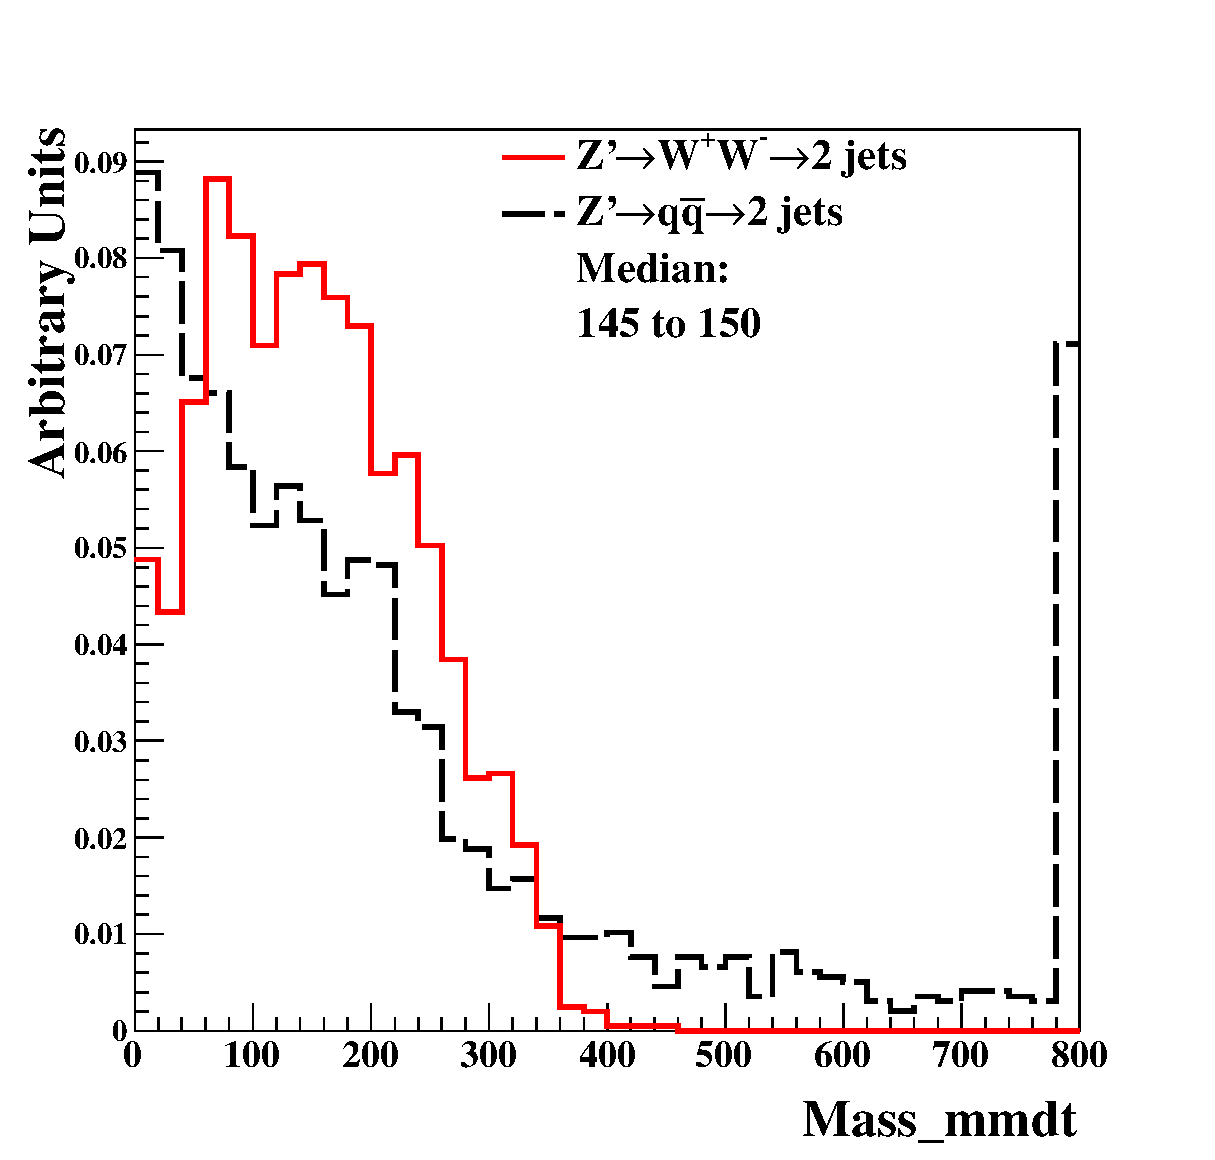
\includegraphics[ width=0.3\textwidth]{h_soft_drop/Dis_cluster_010_mass_mmdt_20tev_04_no_UOF.eps}
   }
      \subfigure[5$\times$5 cm$^2$] {
   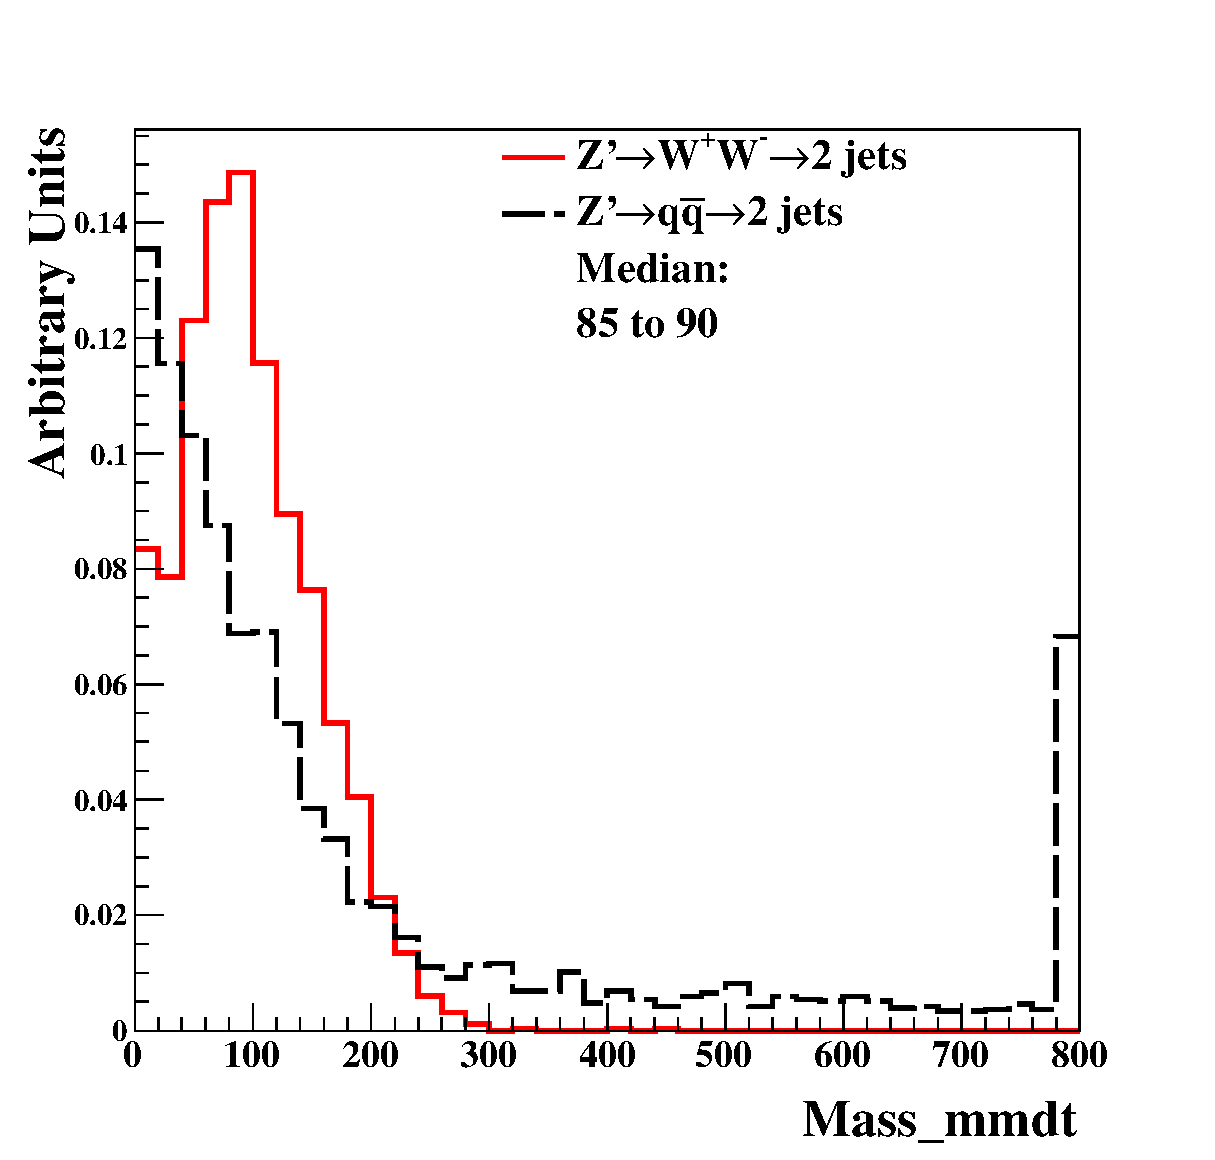
\includegraphics[ width=0.3\textwidth]{h_soft_drop/Dis_cluster_009_mass_mmdt_20tev_04_no_UOF.eps}\hfill
   }
   \subfigure[1$\times$1 cm$^2$] {
   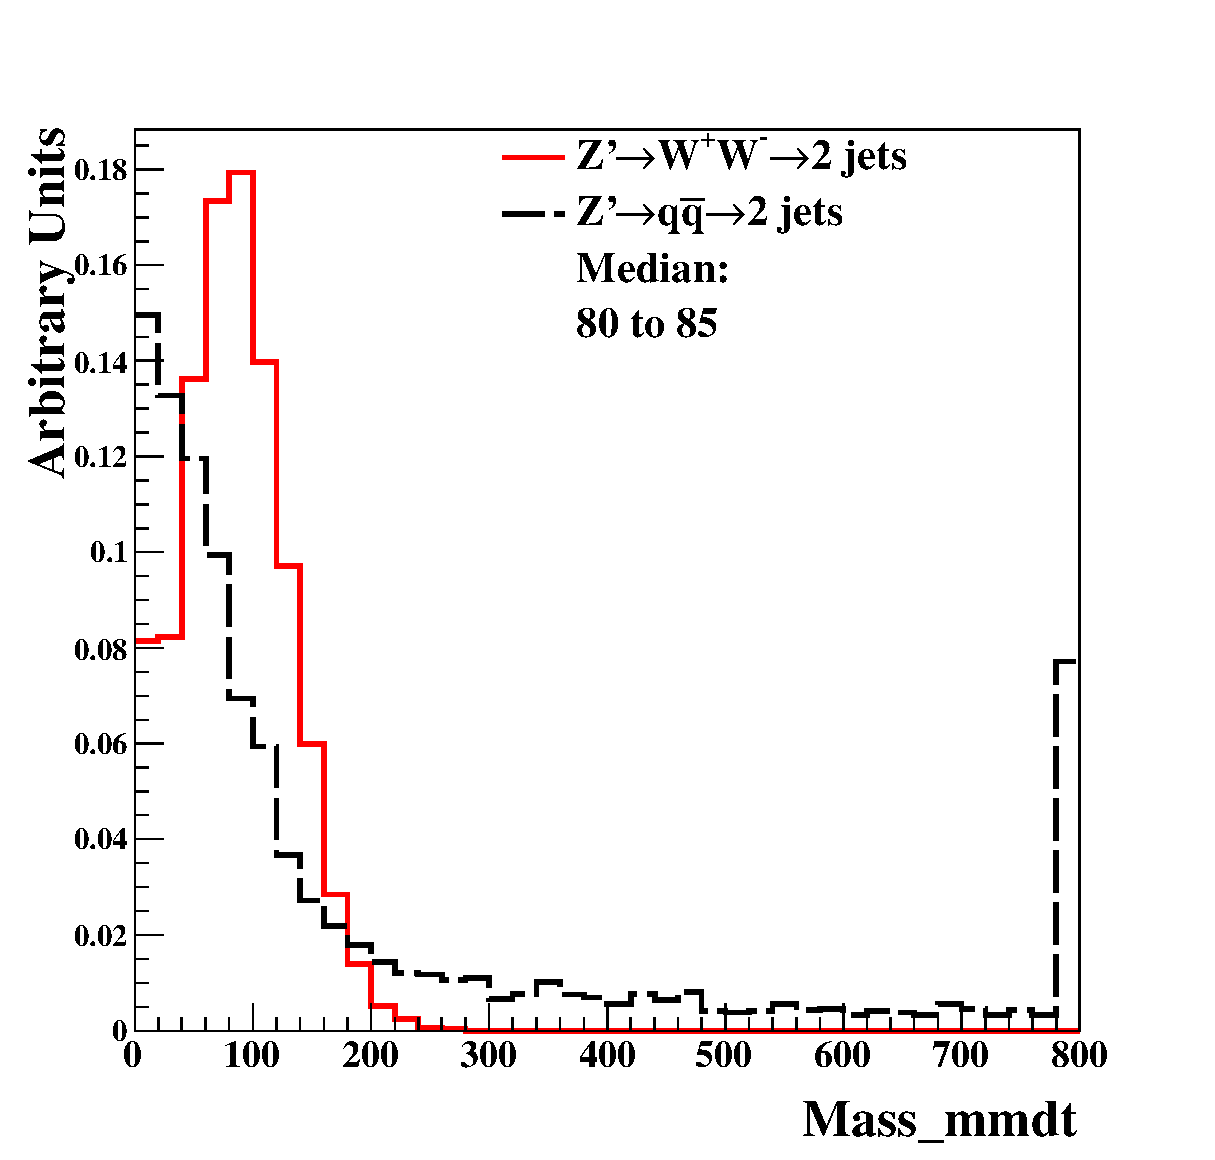
\includegraphics[ width=0.3\textwidth]{h_soft_drop/Dis_cluster_012_mass_mmdt_20tev_04_no_UOF.eps}\hfill
   }
\end{center}
\caption{Distributions of soft drop mass for $\beta$=0, with $M(Z') = 20$~TeV and three different detector cell sizes: 20$\times$20, 
5$\times$5 and 1$\times$1 cm$^2$. The signal (background) process is 
$Z' \rightarrow WW$ ($Z'\rightarrow q\bar{q}$).
\label{fig:cluster_mass_mmdt_ww}}
\end{figure}

\begin{figure}
\begin{center}
  \subfigure[$M(Z')=5$~TeV] {
  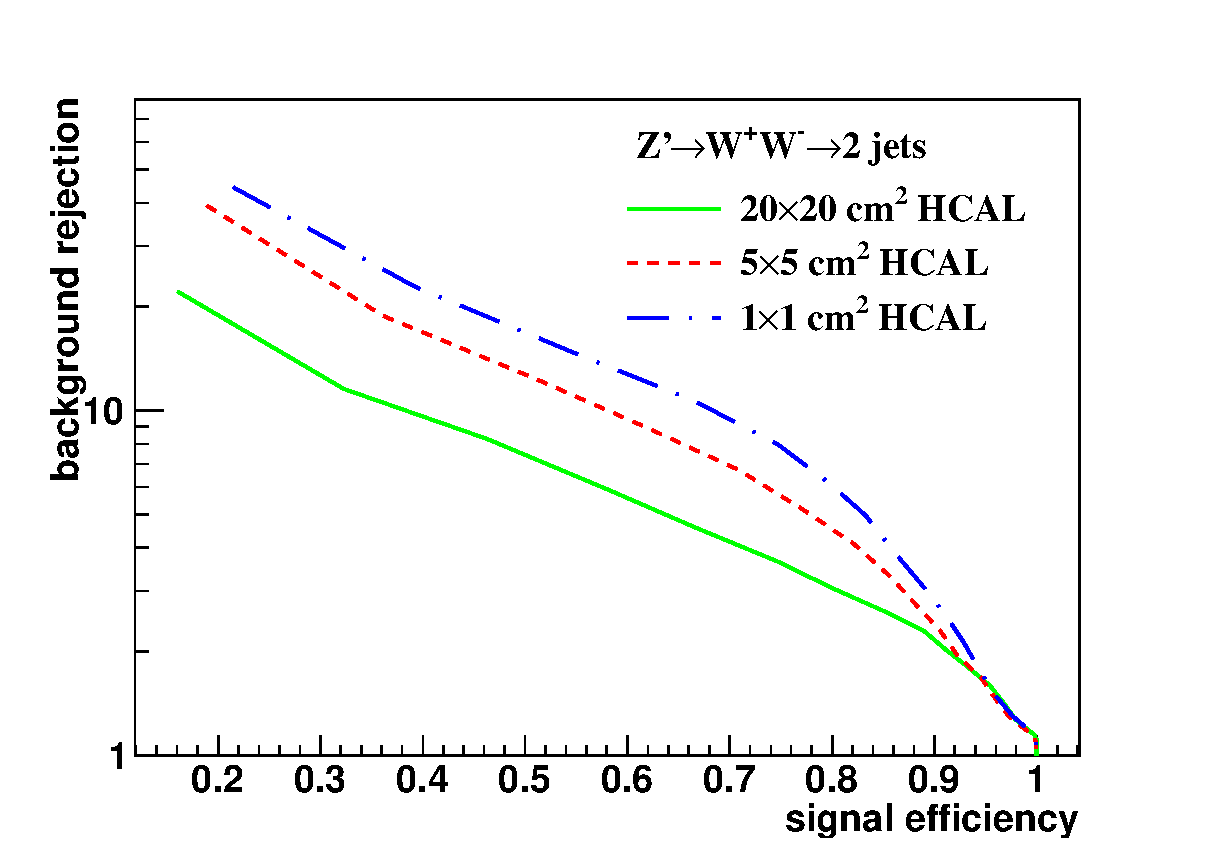
\includegraphics[  width=0.45\textwidth]{ROC_soft_drop/A_Cluster_mass_mmdt_5tev_eff_1_central_fix_at_Median_bin_ww_qq_log_no_UOF.eps}
  }
  \subfigure[$M(Z')=10$~TeV] {
  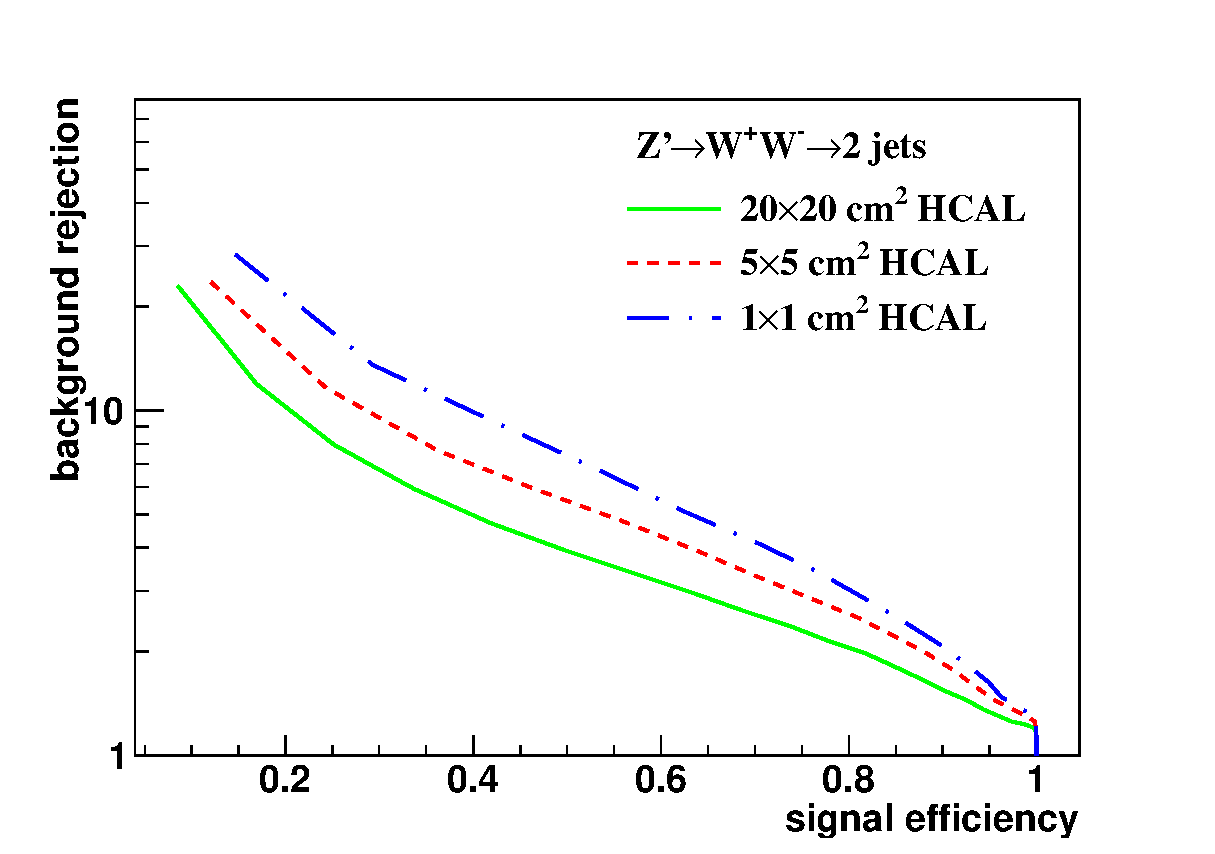
\includegraphics[  width=0.45\textwidth]{ROC_soft_drop/A_Cluster_mass_mmdt_10tev_eff_1_central_fix_at_Median_bin_ww_qq_log_no_UOF.eps}
  }
 \subfigure[$M(Z')=20$~TeV] {
 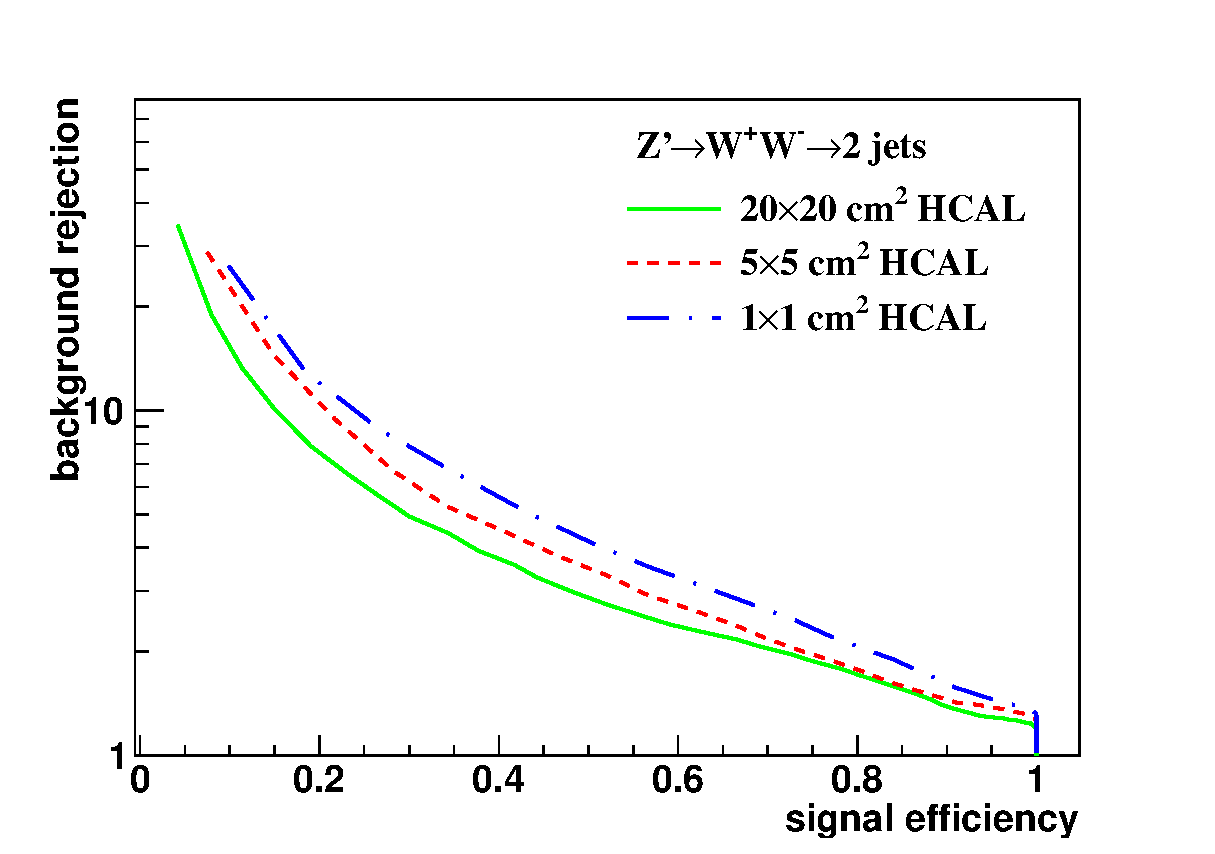
\includegraphics[  width=0.45\textwidth]{ROC_soft_drop/A_Cluster_mass_mmdt_20tev_eff_1_central_fix_at_Median_bin_ww_qq_log_no_UOF.eps}
 }
 \subfigure[$M(Z')=40$~TeV] {
 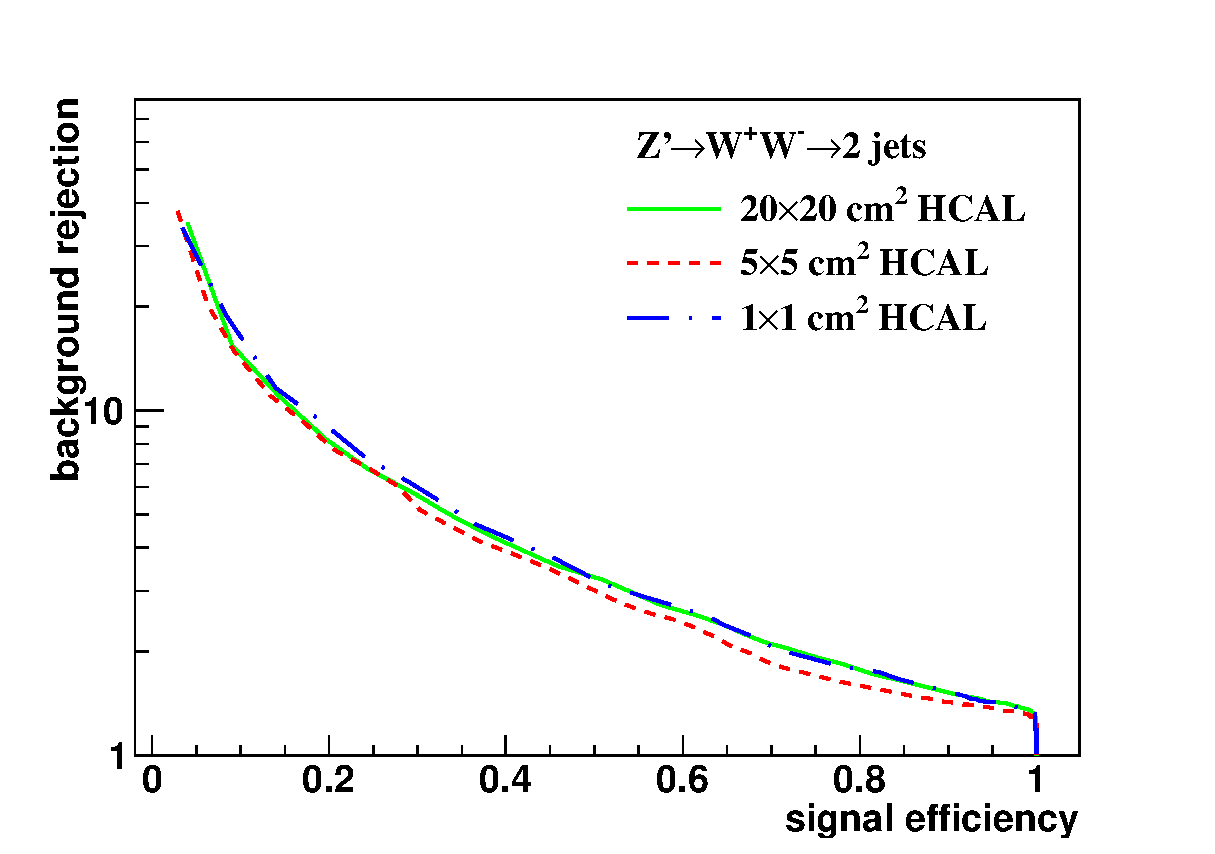
\includegraphics[  width=0.45\textwidth]{ROC_soft_drop/A_Cluster_mass_mmdt_40tev_eff_1_central_fix_at_Median_bin_ww_qq_log_no_UOF.eps}
 }
\end{center}
\caption{The ROC curves of soft drop mass selection for $\beta$=0 
with resonance masses of 5, 10, 20 and 40 TeV. 
Three different detector cell sizes are compared: 20~$ \times $~20, 
5~$ \times $~5, and 1~$ \times $~1 cm$^2$. 
The signal (background) process is $Z'\rightarrow WW$ 
($Z' \rightarrow q\bar{q}$).}
\label{fig:cluster_mass_mmdt_ww_ROC}
\end{figure}

\begin{figure}
\begin{center}
   \subfigure[5~$\times$~5 cm$^2$] {
   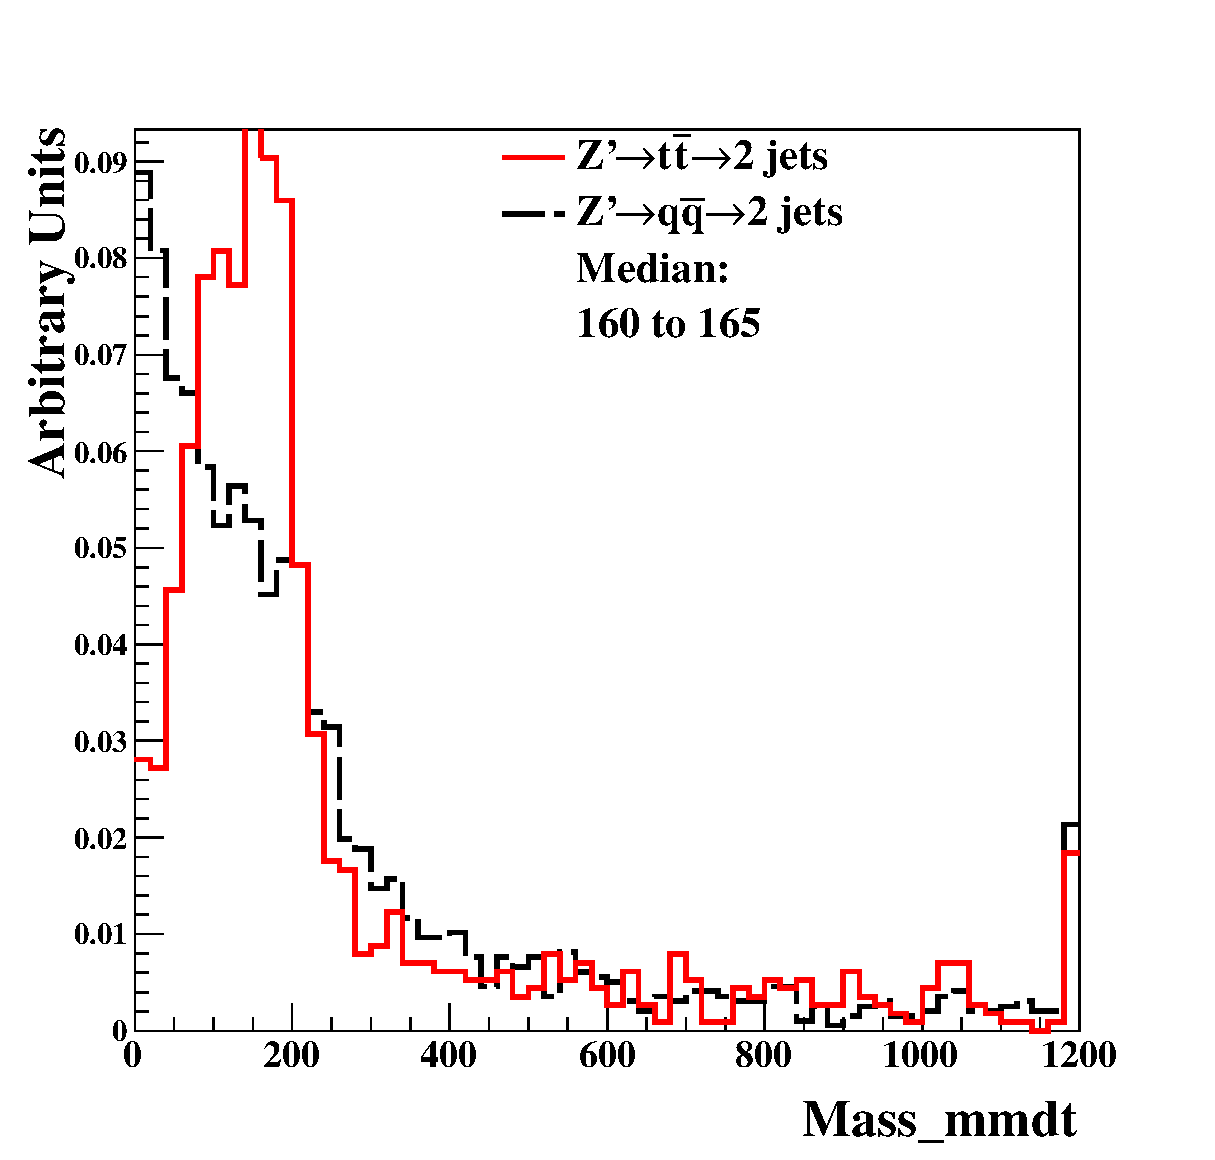
\includegraphics[   width=0.3\textwidth]{h_soft_drop/Dis_cluster_010_mass_mmdt_tt_20tev_04_tt_no_UOF.eps}
   }
   \subfigure[20~$\times$~20 cm$^2$] {
   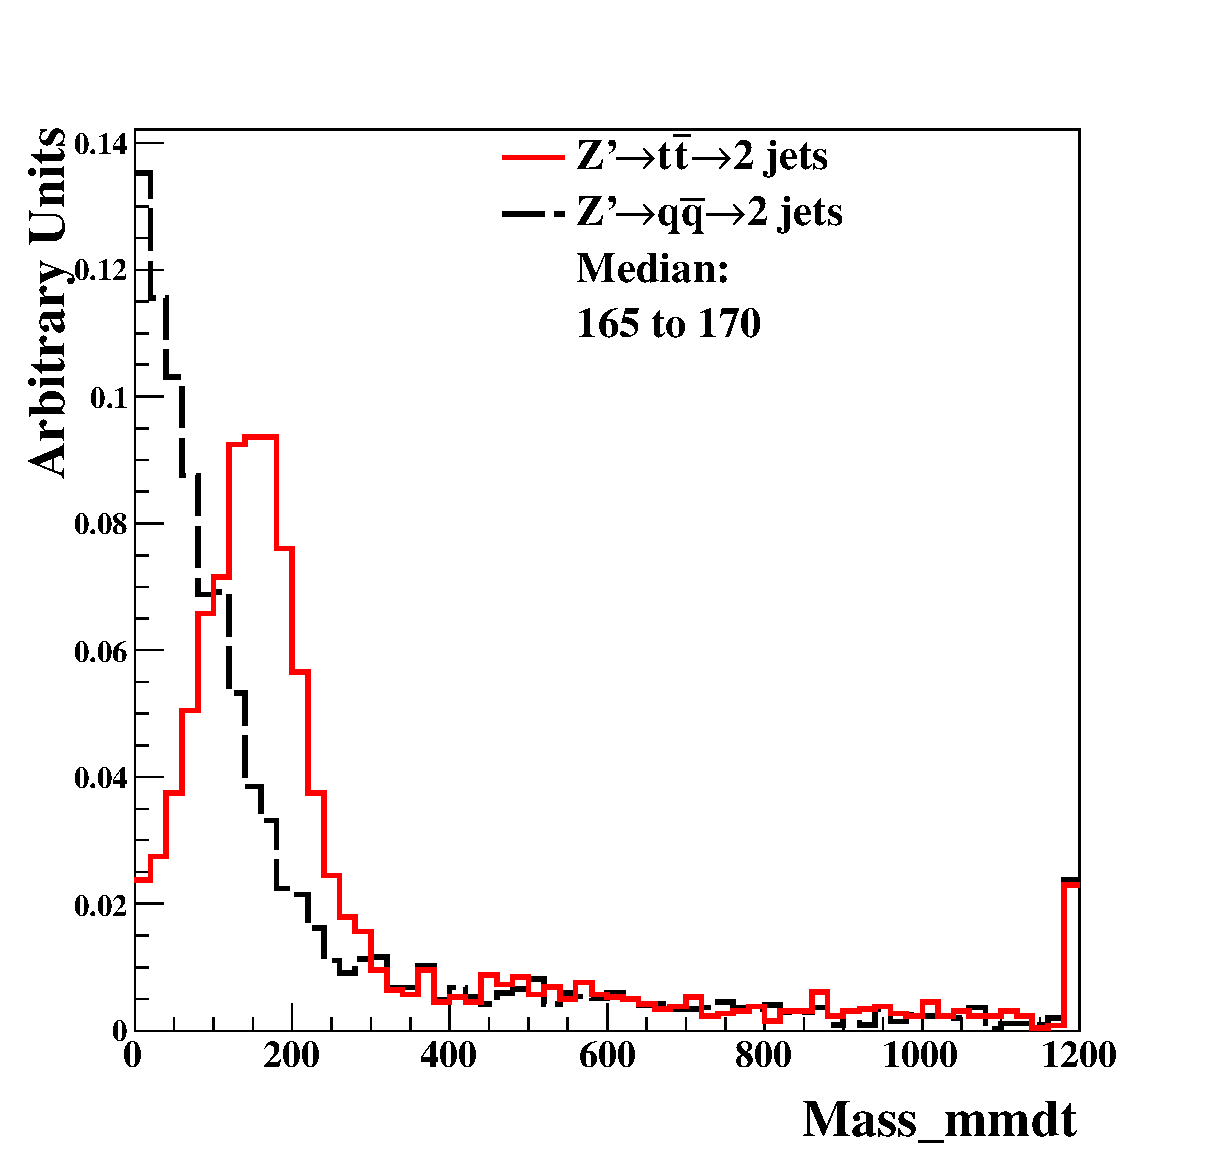
\includegraphics[   width=0.3\textwidth]{h_soft_drop/Dis_cluster_009_mass_mmdt_tt_20tev_04_tt_no_UOF.eps}\hfill
   }
   \subfigure[1~$\times$~1 cm$^2$] {
   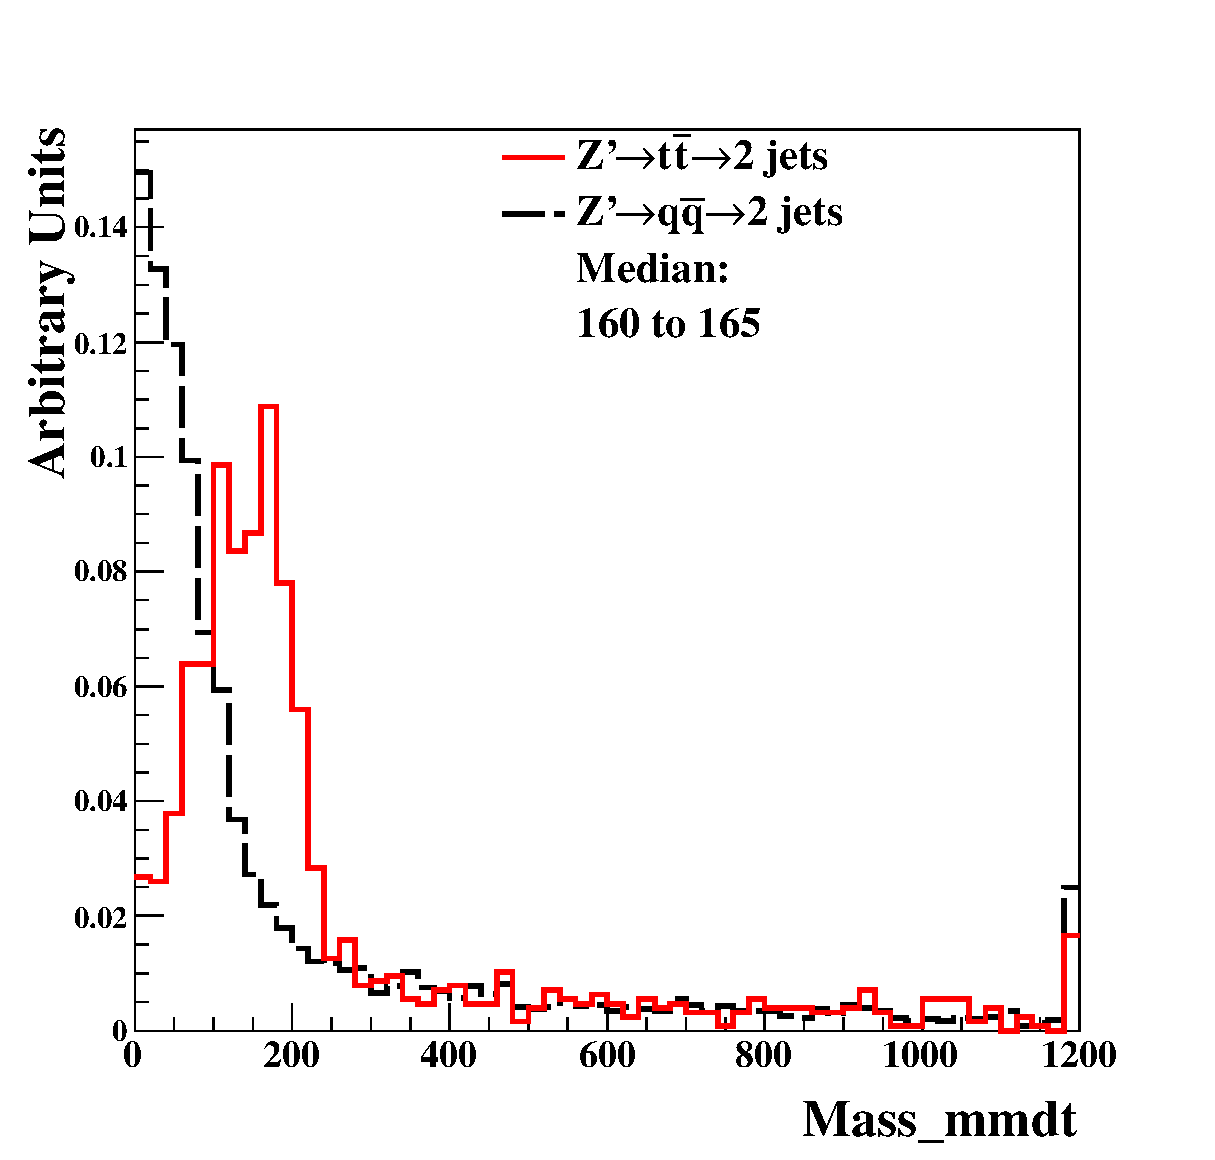
\includegraphics[   width=0.3\textwidth]{h_soft_drop/Dis_cluster_012_mass_mmdt_tt_20tev_04_tt_no_UOF.eps}\hfill
   }
\end{center}
\caption{
Distributions of soft drop mass for $\beta$=0, with $M(Z') = 20$~TeV  and three different detector cell sizes: 20~$\times$~20, 
5~$\times$~5, and 1~$\times$~1 cm$^2$. The signal (background) process is 
$Z' \rightarrow t\bar{t}$ ($Z'\rightarrow q\bar{q}$).
}
\label{fig:cluster_mass_mmdt_tt}
\end{figure}


\begin{figure}
\begin{center}
  \subfigure[$M(Z')=5$~TeV] {
  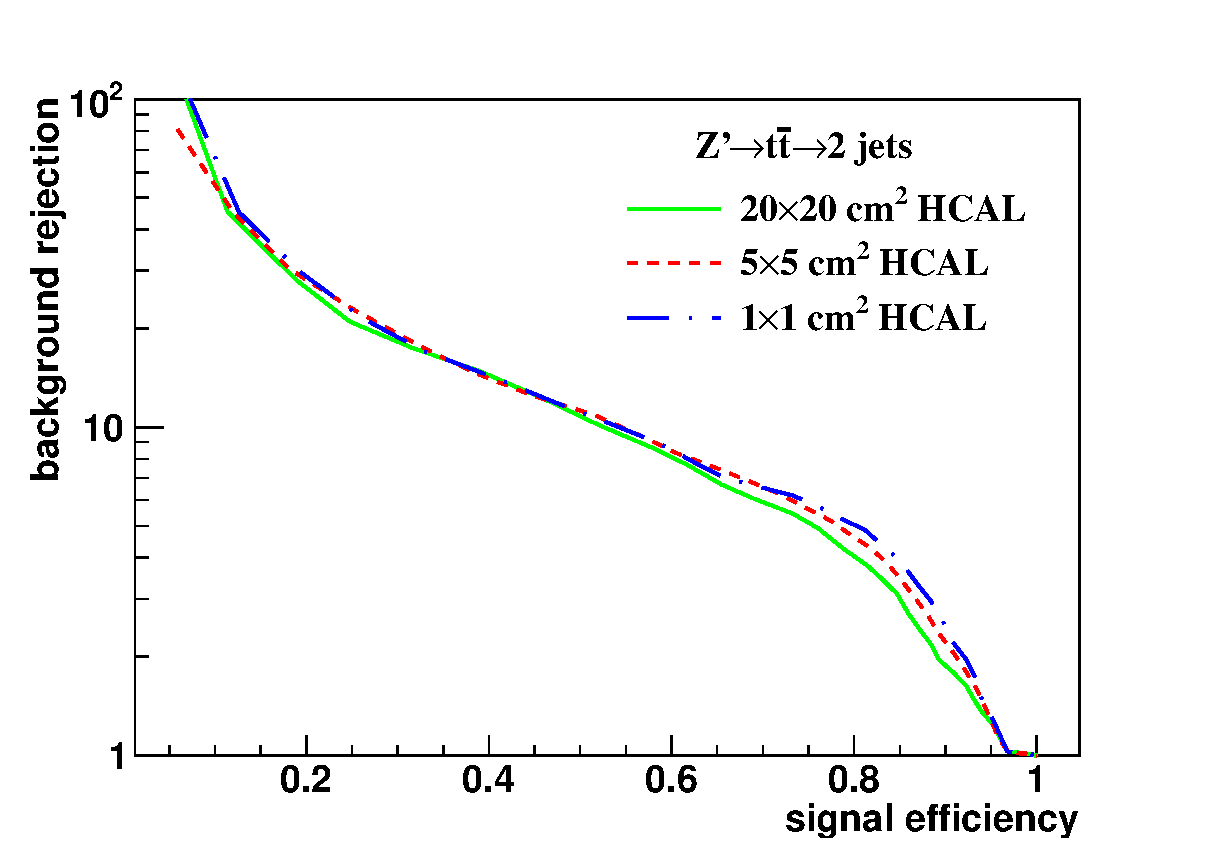
\includegraphics[  width=0.45\textwidth]{ROC_soft_drop/A_Cluster_mass_mmdt_5tev_eff_1_central_fix_at_Median_bin_tt_qq_log_no_UOF.eps}
  }
  \subfigure[$M(Z')=10$~TeV] {
  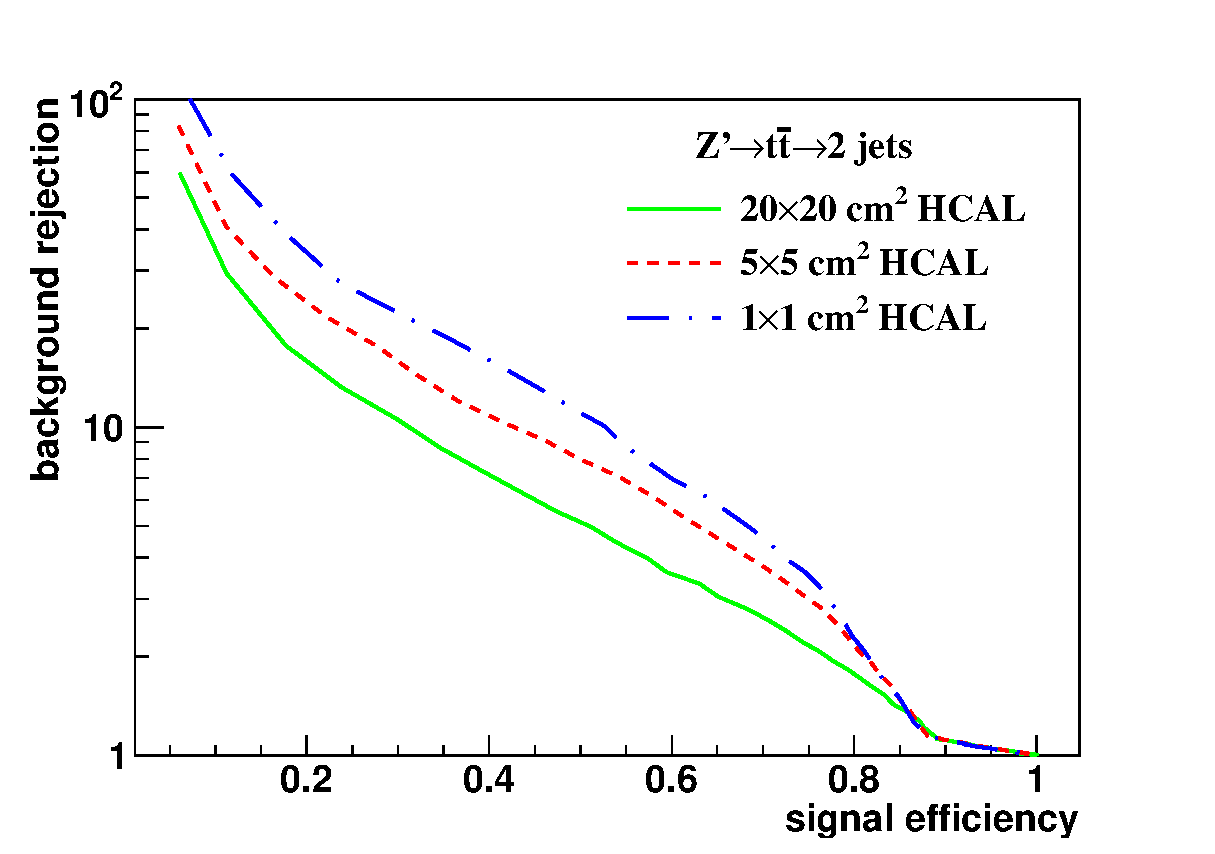
\includegraphics[  width=0.45\textwidth]{ROC_soft_drop/A_Cluster_mass_mmdt_10tev_eff_1_central_fix_at_Median_bin_tt_qq_log_no_UOF.eps}
  }
 \subfigure[$M(Z')=20$~TeV] {
 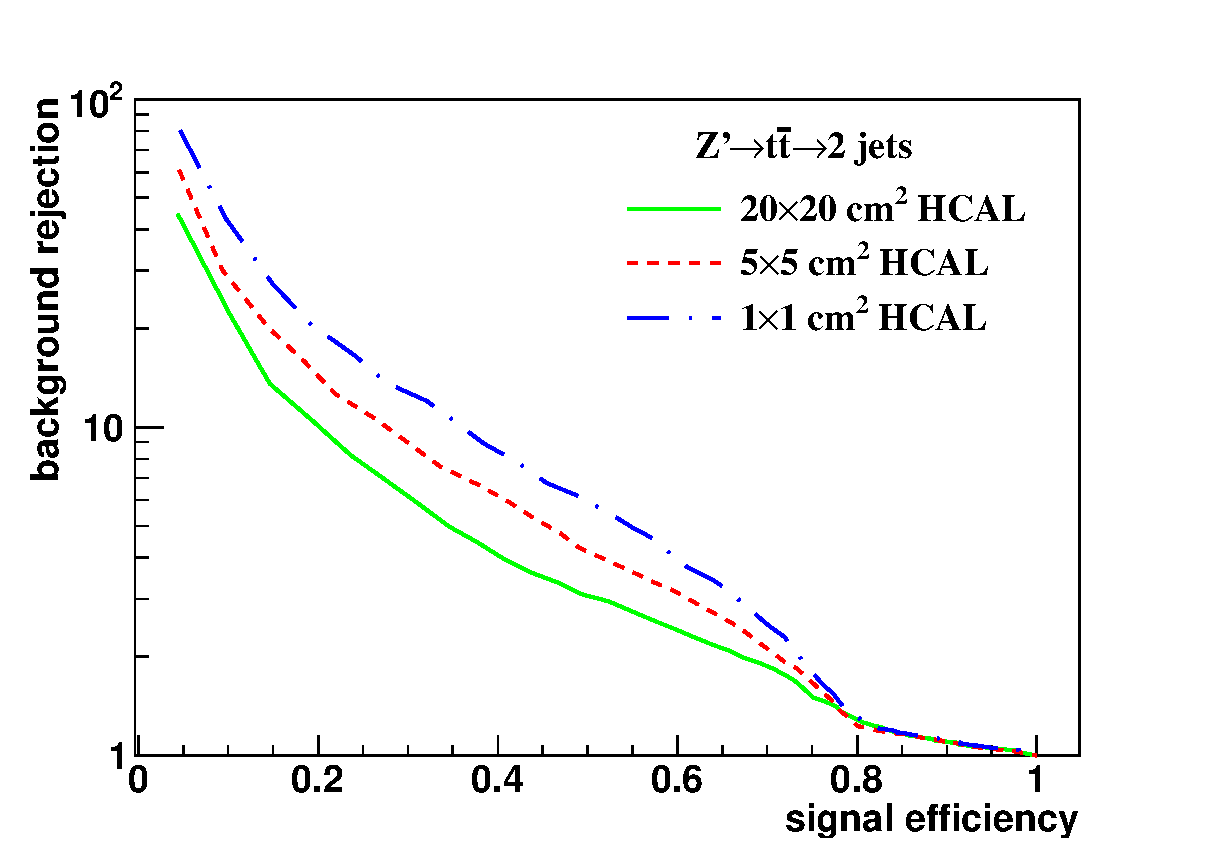
\includegraphics[  width=0.45\textwidth]{ROC_soft_drop/A_Cluster_mass_mmdt_20tev_eff_1_central_fix_at_Median_bin_tt_qq_log_no_UOF.eps}
 }
 \subfigure[$M(Z')=40$~TeV] {
 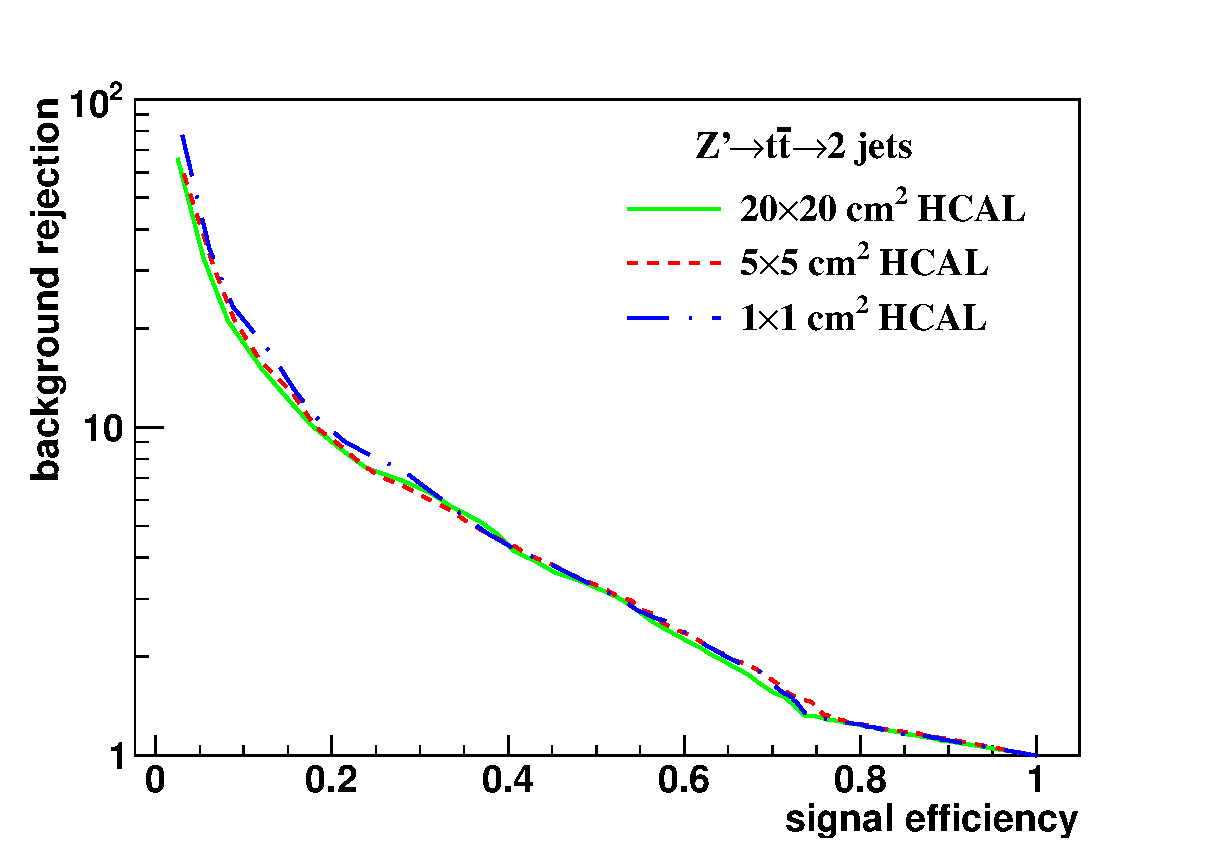
\includegraphics[  width=0.45\textwidth]{ROC_soft_drop/A_Cluster_mass_mmdt_40tev_eff_1_central_fix_at_Median_bin_tt_qq_log_no_UOF.eps}
 }
\end{center}
\caption{
The ROC curves of soft drop mass selection for $\beta$=0 
with resonance masses of 5, 10, 20 and 40 TeV. 
Three different detector cell sizes are compared: 20~$\times$~20, 
5~$\times$~5, and 1~$\times$~1 cm$^2$. 
The signal (background) process is $Z'\rightarrow t\bar{t}$
($Z' \rightarrow q\bar{q}$).
}
\label{fig:cluster_mass_mmdt_tt_ROC}
\end{figure}

\begin{figure}
\begin{center}
   \subfigure[20~$\times$~20 cm$^2$] {
   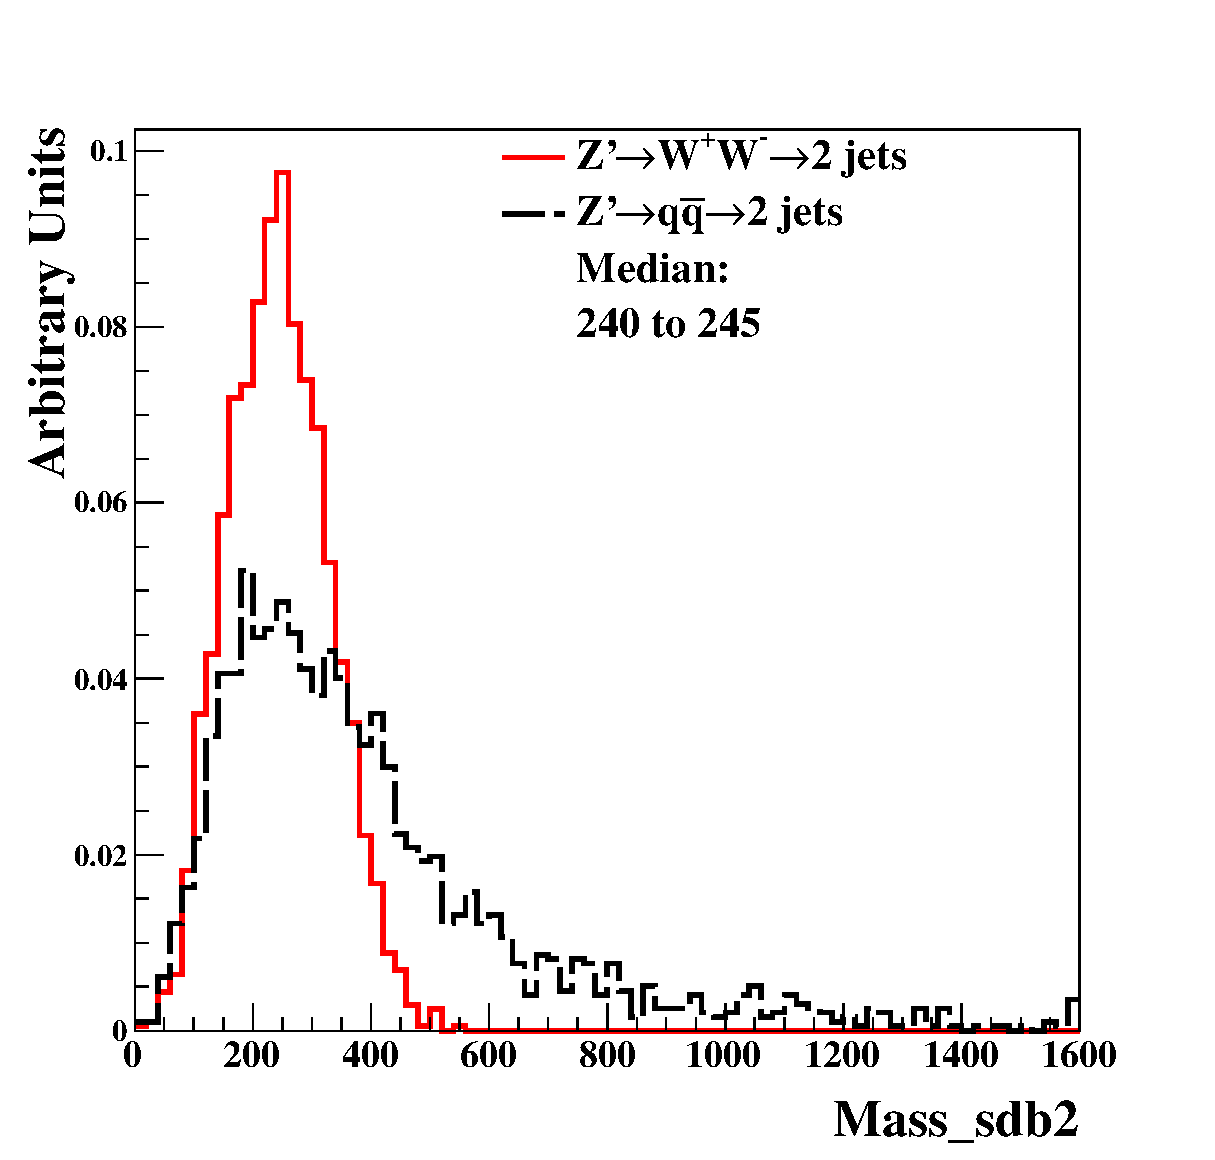
\includegraphics[   width=0.3\textwidth]{h_soft_drop/Dis_cluster_010_mass_sdb2_ww_20tev_04_1600_no_UOF.eps}
   }
    \subfigure[5~$\times$~5 cm$^2$] {
   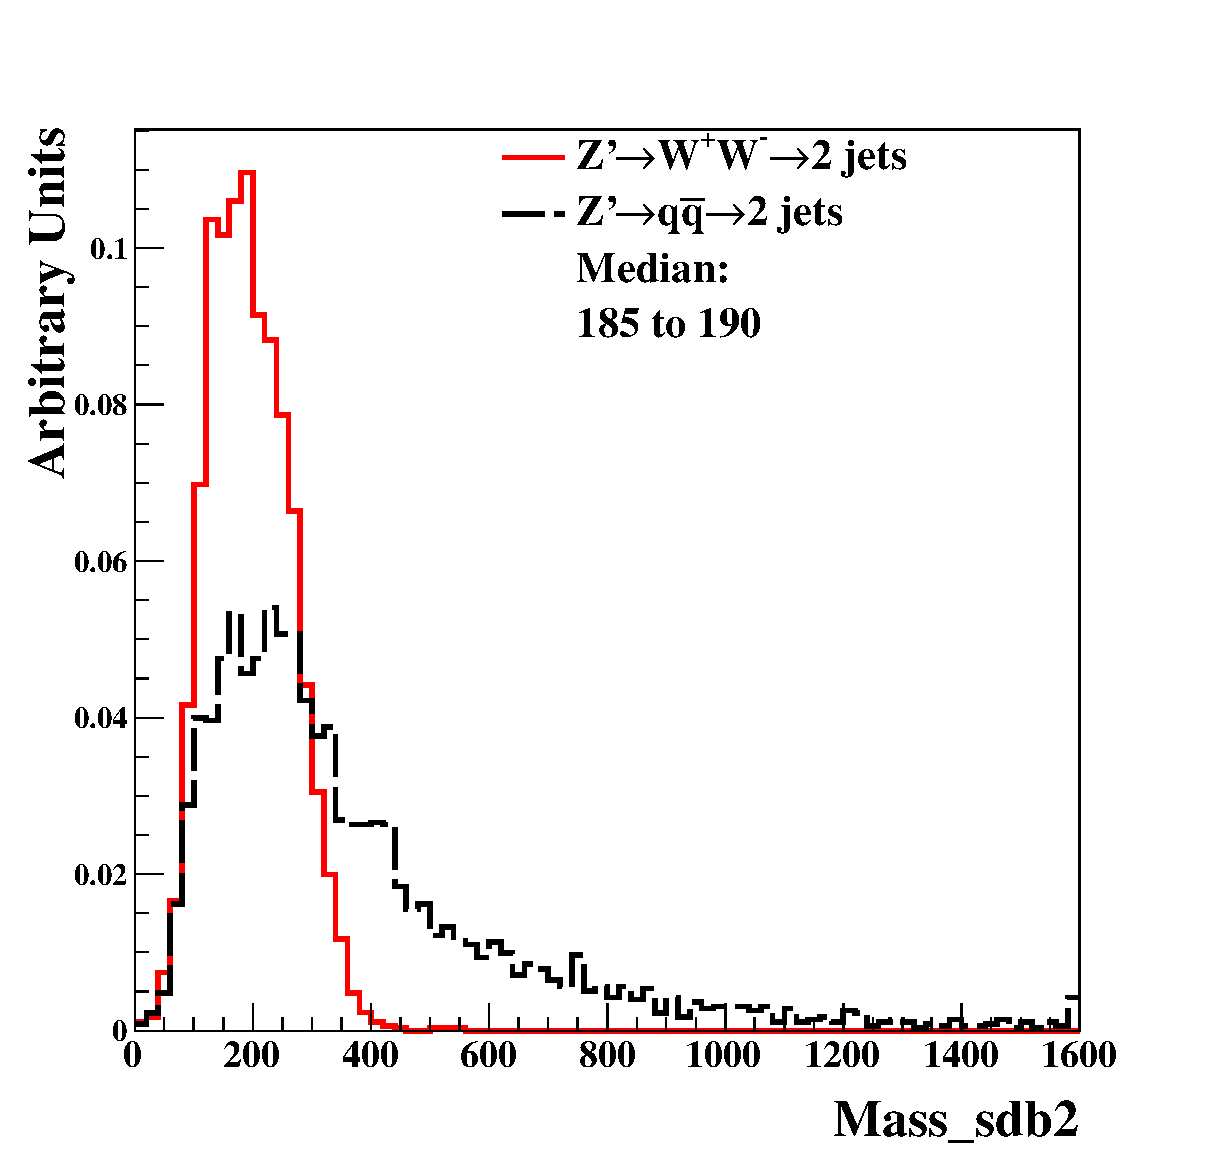
\includegraphics[   width=0.3\textwidth]{h_soft_drop/Dis_cluster_009_mass_sdb2_ww_20tev_04_1600_no_UOF.eps}\hfill
   }
   \subfigure[1~$\times$~1 cm$^2$] {
   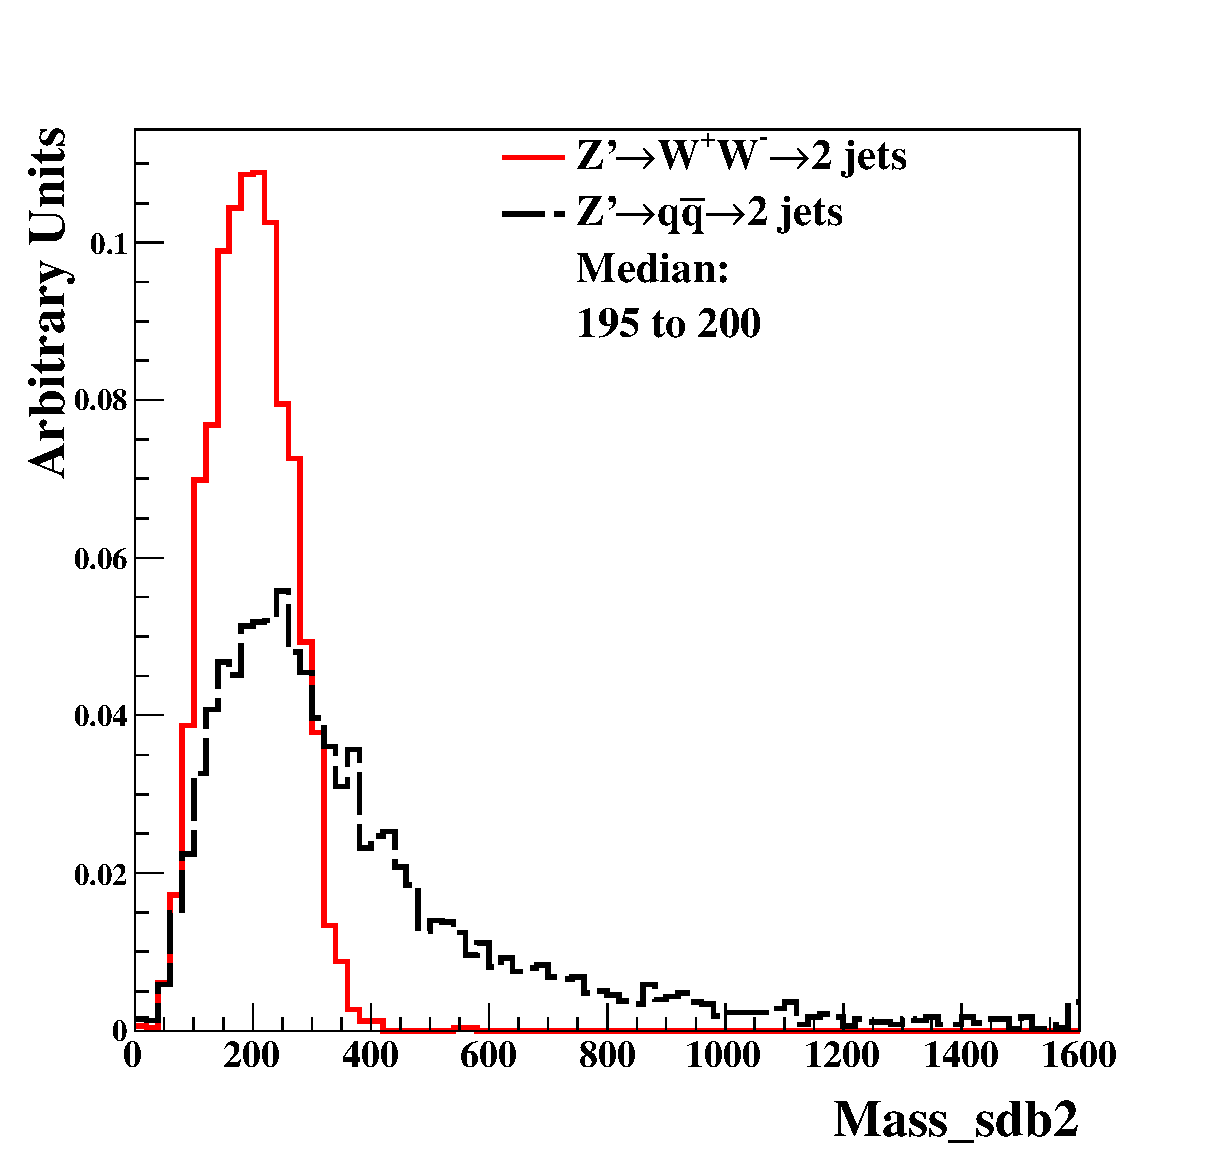
\includegraphics[   width=0.3\textwidth]{h_soft_drop/Dis_cluster_012_mass_sdb2_ww_20tev_04_1600_no_UOF.eps}\hfill
   }
\end{center}
\caption{
Distributions of soft drop mass for $\beta=2$, with $M(Z') = 20 $~TeV  and three different detector cell sizes: 20~$\times$~20, 
5~$\times$~5 and 1~$\times$~1 cm$^2$. The signal (background) process is 
$Z'\rightarrow WW$ ($Z'\rightarrow q\bar{q}$).
}
\label{fig:cluster_mass_sdb2_ww}
\end{figure}


\begin{figure}
\begin{center}
  \subfigure[$M(Z')=5$~TeV] {
  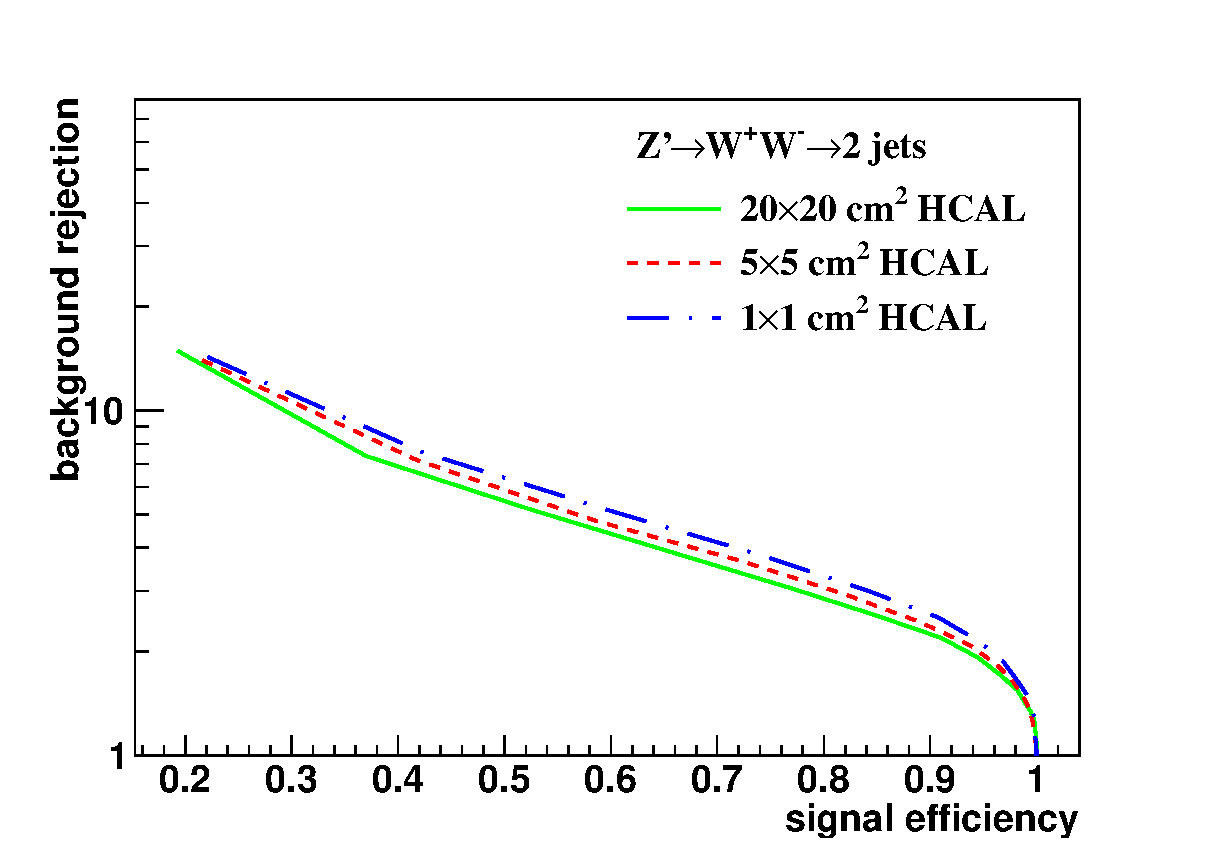
\includegraphics[  width=0.45\textwidth]{ROC_soft_drop/A_Cluster_mass_sdb2_5tev_eff_1_central_fix_at_Median_bin_ww_qq_log_no_UOF.eps}
  }
  \subfigure[$M(Z')=10$~TeV] {
  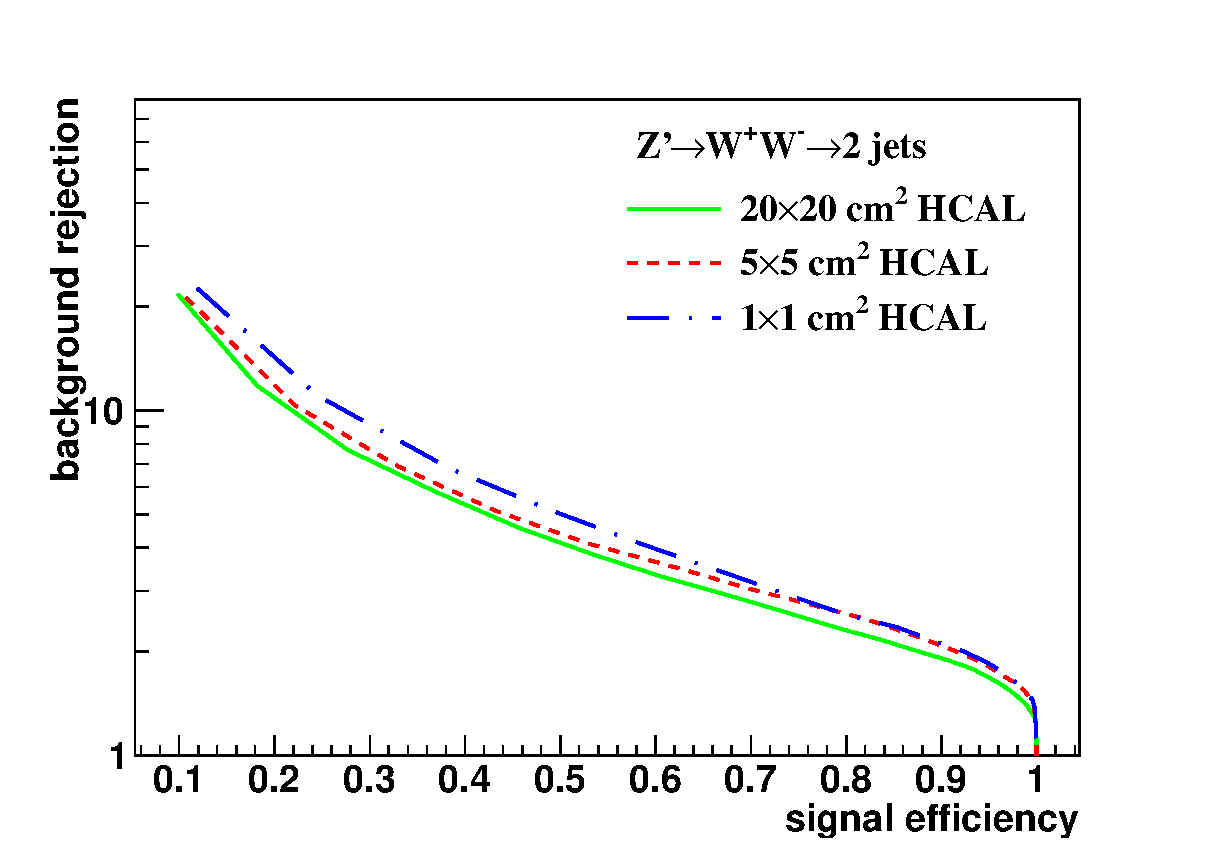
\includegraphics[  width=0.45\textwidth]{ROC_soft_drop/A_Cluster_mass_sdb2_10tev_eff_1_central_fix_at_Median_bin_ww_qq_log_no_UOF.eps}
  }
 \subfigure[$M(Z')=20$~TeV] {
 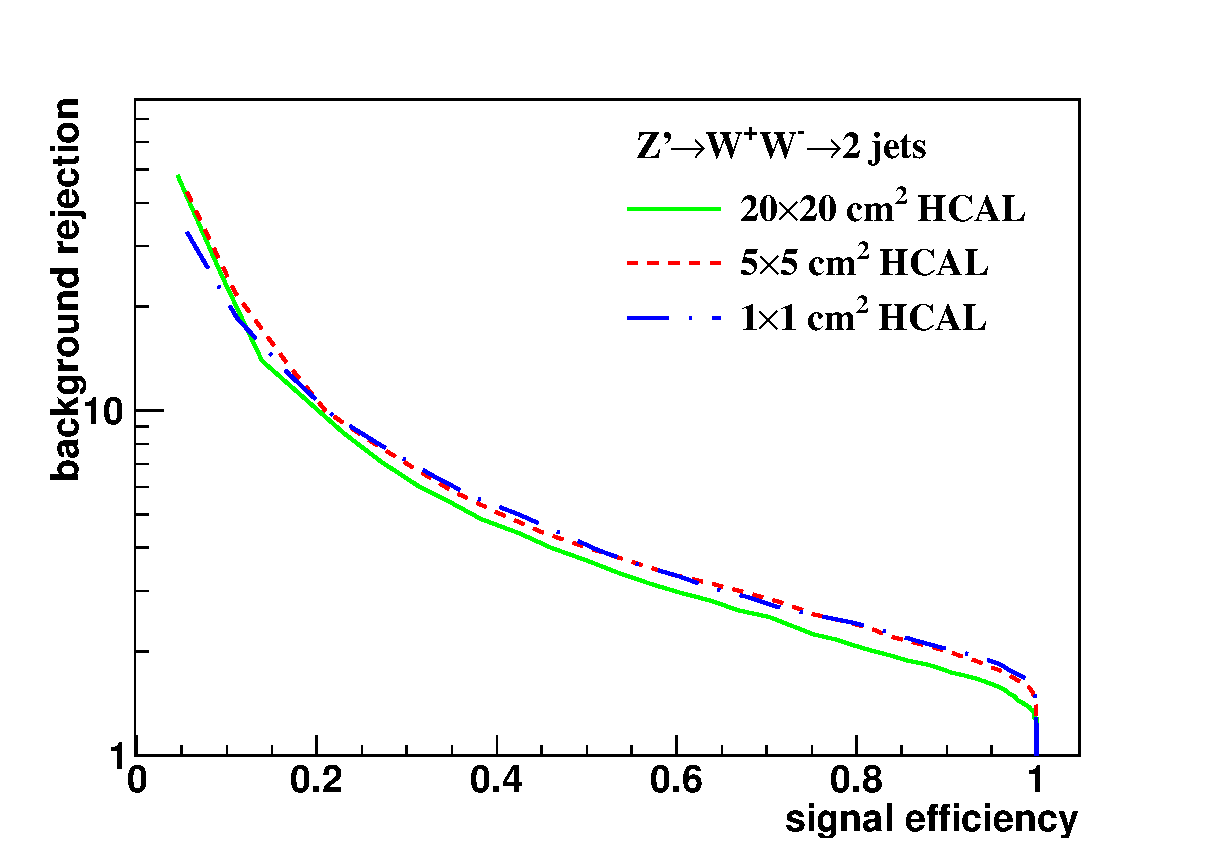
\includegraphics[  width=0.45\textwidth]{ROC_soft_drop/A_Cluster_mass_sdb2_20tev_eff_1_central_fix_at_Median_bin_ww_qq_log_no_UOF.eps}
 }
 \subfigure[$M(Z')=40$~TeV] {
 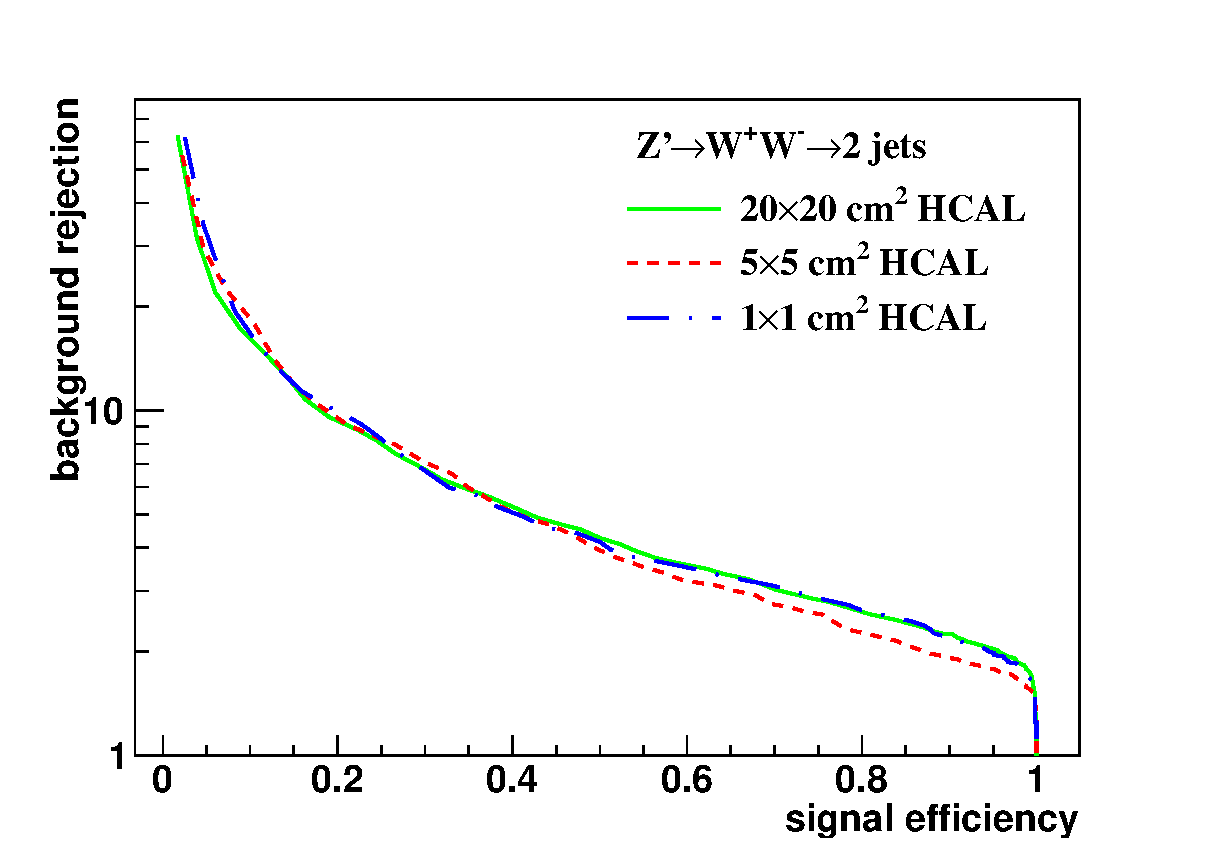
\includegraphics[  width=0.45\textwidth]{ROC_soft_drop/A_Cluster_mass_sdb2_40tev_eff_1_central_fix_at_Median_bin_ww_qq_log_no_UOF.eps}
 }
\end{center}
\caption{
The ROC curves of soft drop mass selection for $\beta=2$
with resonance masses of 5, 10, 20 and 40 TeV. 
Three different detector cell sizes are compared: 20~$\times$~20, 
5~$\times$~5, and 1~$\times$~1 cm$^2$. 
The signal (background) process is $Z'\rightarrow WW$ 
($Z'\rightarrow q\bar{q}$).}
\label{fig:cluster_mass_sdb2_ww_ROC}
\end{figure}

\begin{figure}
\begin{center}
   \subfigure[20~$\times$~20 cm$^2$] {
   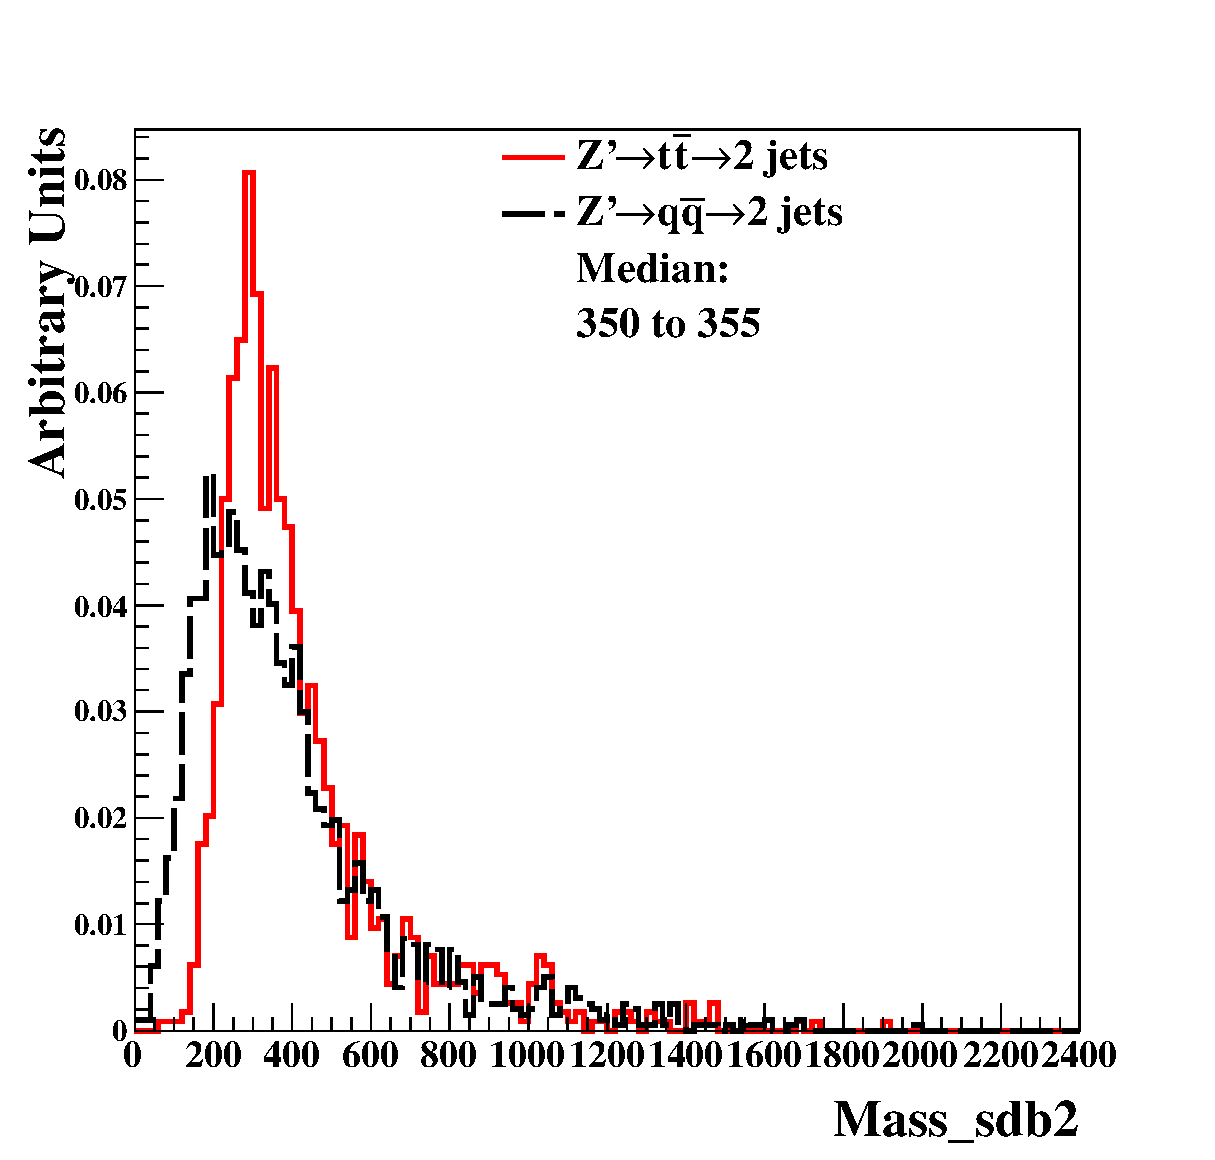
\includegraphics[   width=0.3\textwidth]{h_soft_drop/Dis_cluster_010_mass_sdb2_tt_20tev_04_tt_2400_no_UOF.eps}
   }
   \subfigure[5~$\times$~5 cm$^2$] {
   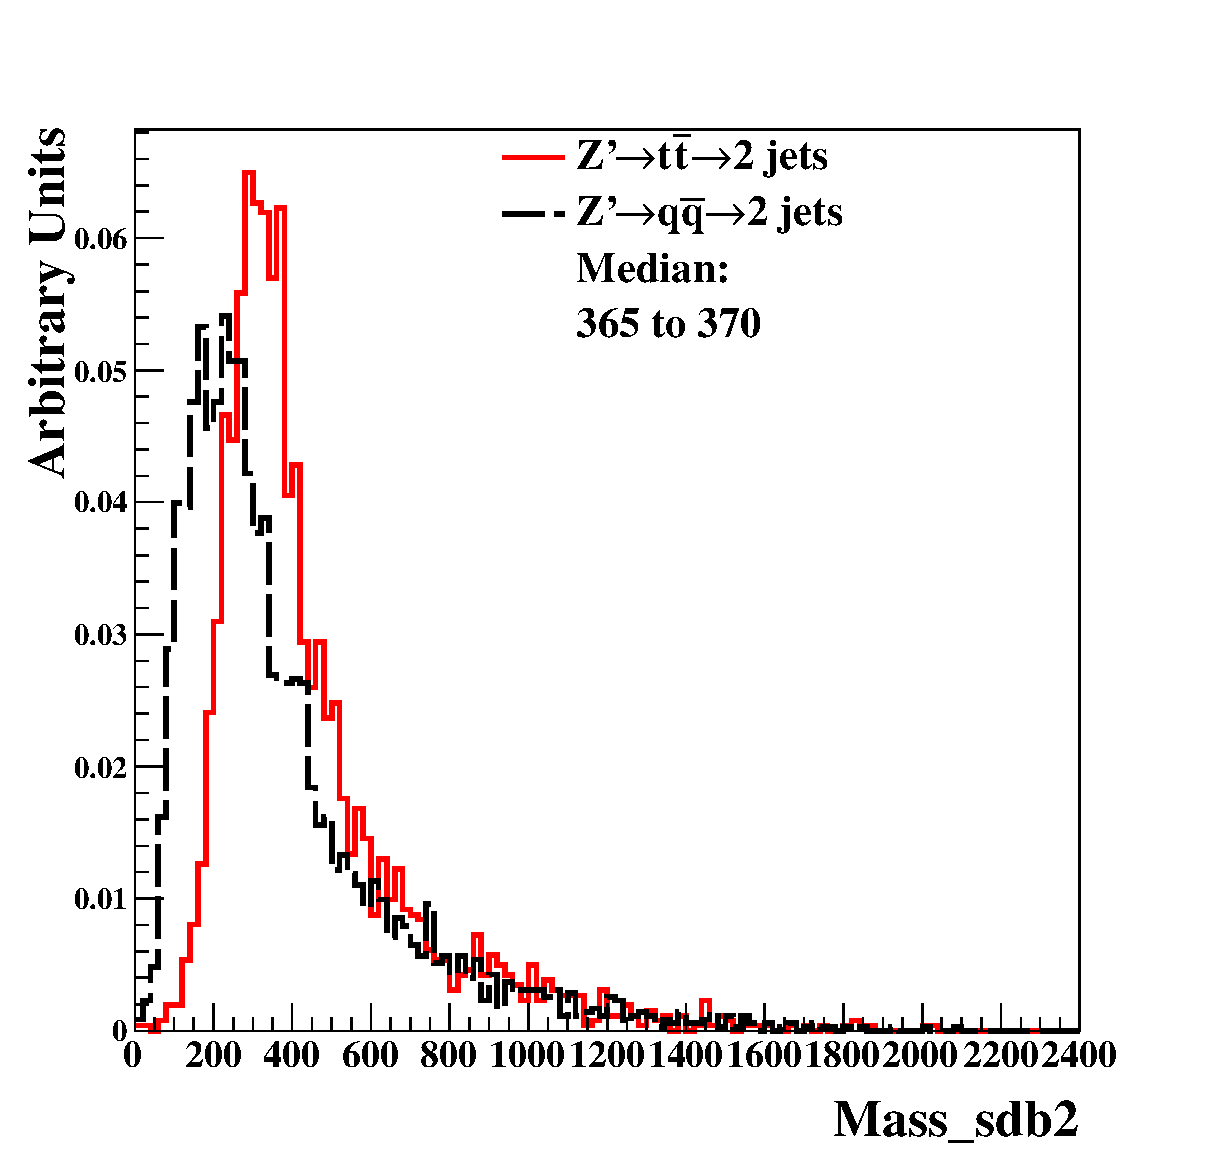
\includegraphics[   width=0.3\textwidth]{h_soft_drop/Dis_cluster_009_mass_sdb2_tt_20tev_04_tt_2400_no_UOF.eps}\hfill
   }
   \subfigure[1~$\times$~1 cm$^2$] {
   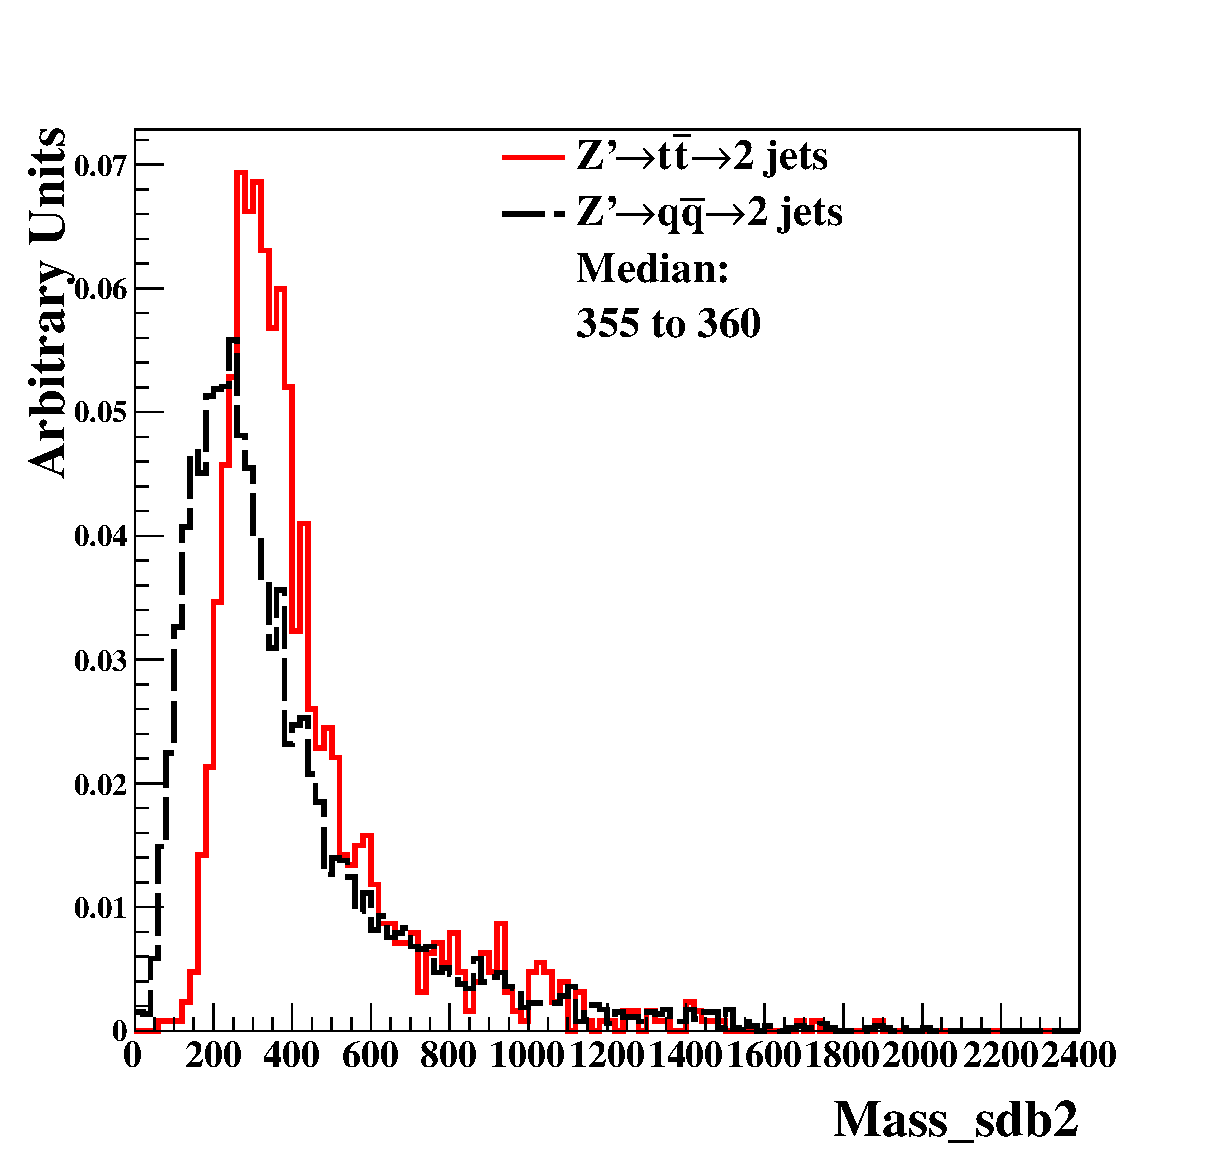
\includegraphics[   width=0.3\textwidth]{h_soft_drop/Dis_cluster_012_mass_sdb2_tt_20tev_04_tt_2400_no_UOF.eps}\hfill
   }
\end{center}
\caption{
Distributions of soft drop mass for $\beta =2$, with $M(Z') =20$~TeV  and three different detector cell sizes: 20~$\times$~20, 
5~$\times$~5, and 1~$\times$~1 cm$^2$. The signal (background) process is  
$Z'\rightarrow t\bar{t}$ ($Z'\rightarrow q\bar{q}$).
}
\label{fig:cluster_mass_sdb2_tt}
\end{figure}


\begin{figure}
\begin{center}
  \subfigure[$M(Z')=5$~TeV] {
  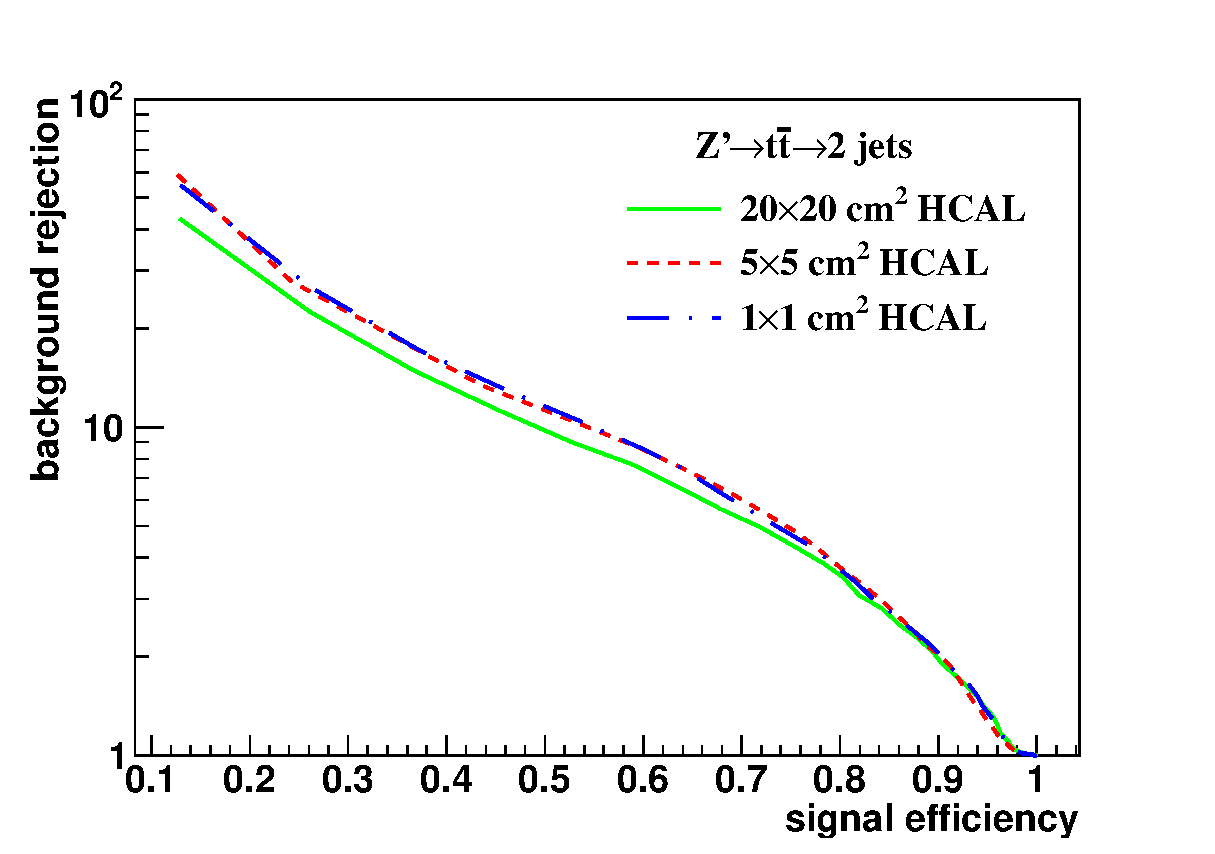
\includegraphics[  width=0.45\textwidth]{ROC_soft_drop/A_Cluster_mass_sdb2_5tev_eff_1_central_fix_at_Median_bin_tt_qq_log_no_UOF.eps}
  }
  \subfigure[$M(Z')=10$~TeV] {
  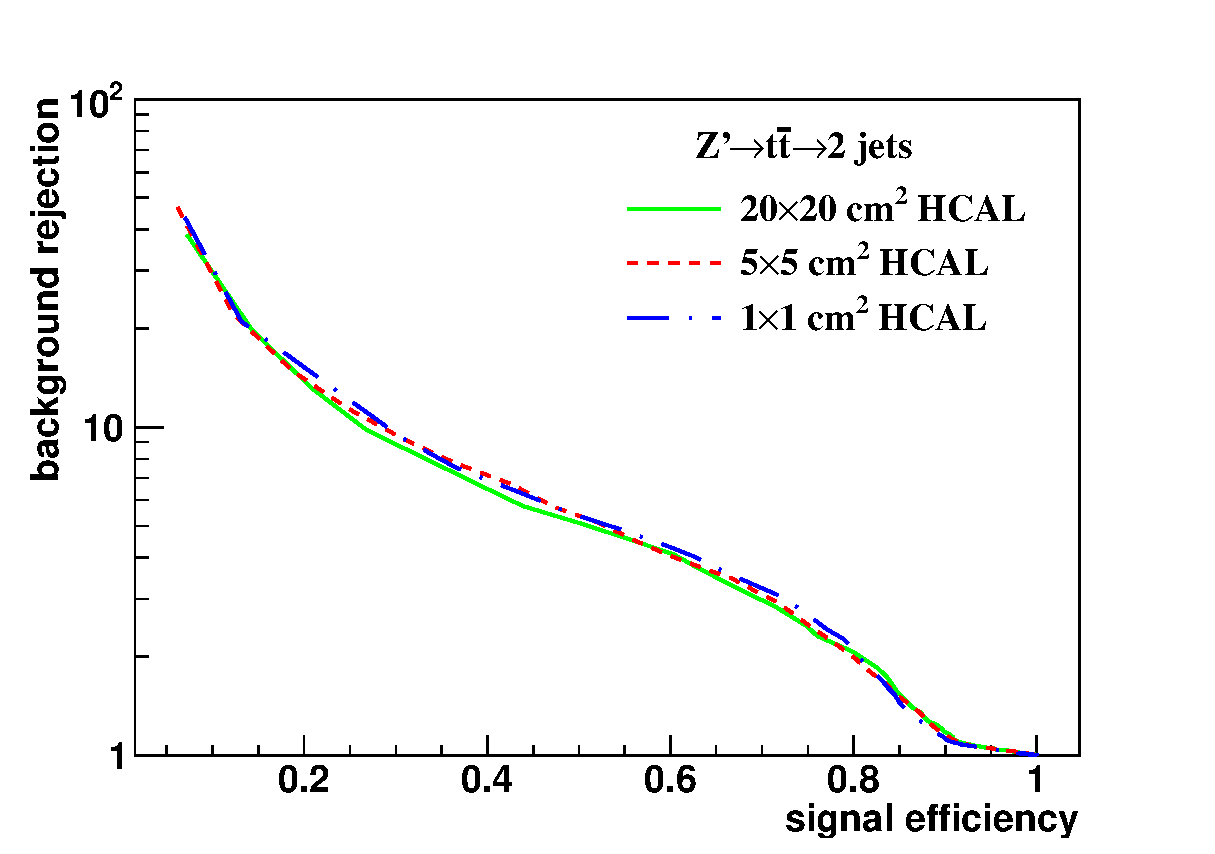
\includegraphics[  width=0.45\textwidth]{ROC_soft_drop/A_Cluster_mass_sdb2_10tev_eff_1_central_fix_at_Median_bin_tt_qq_log_no_UOF.eps}
  }
 \subfigure[$M(Z')=20$~TeV] {
 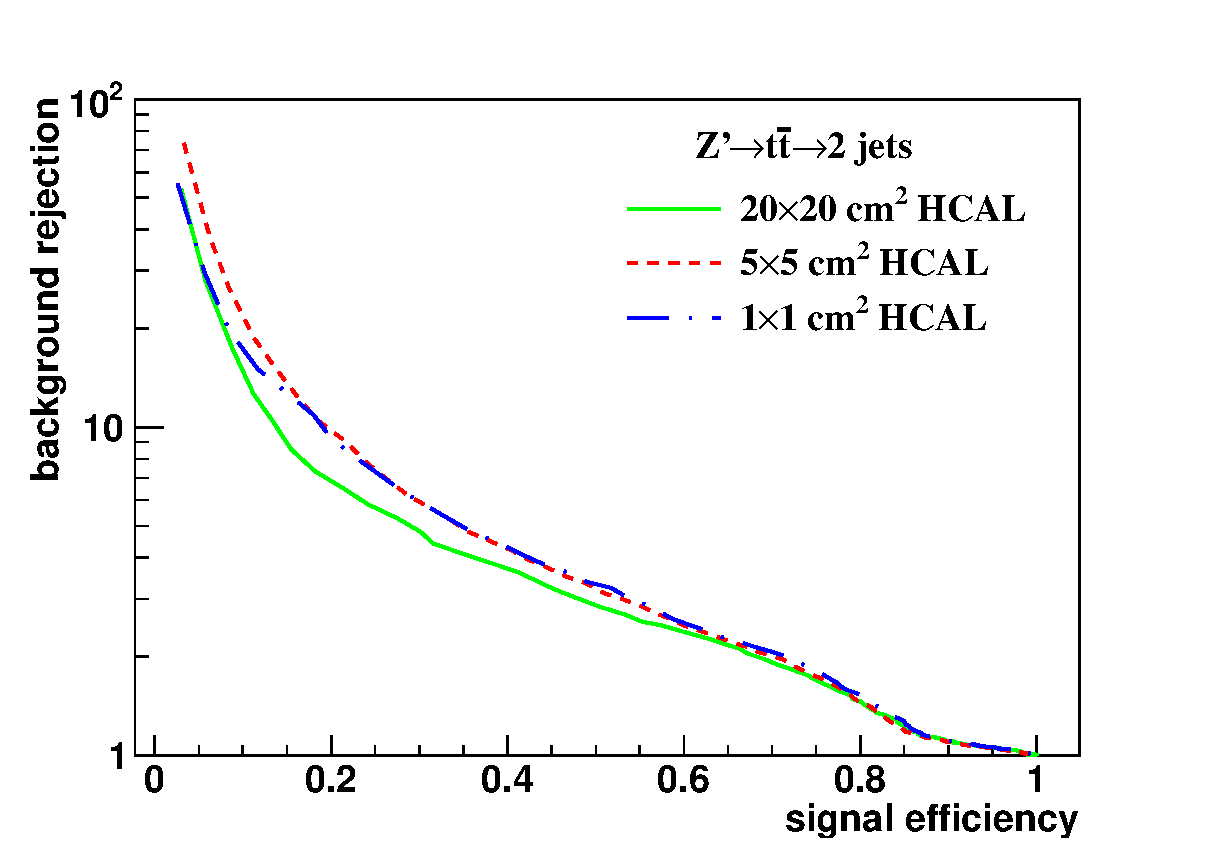
\includegraphics[  width=0.45\textwidth]{ROC_soft_drop/A_Cluster_mass_sdb2_20tev_eff_1_central_fix_at_Median_bin_tt_qq_log_no_UOF.eps}
 }
 \subfigure[$M(Z')=40$~TeV] {
 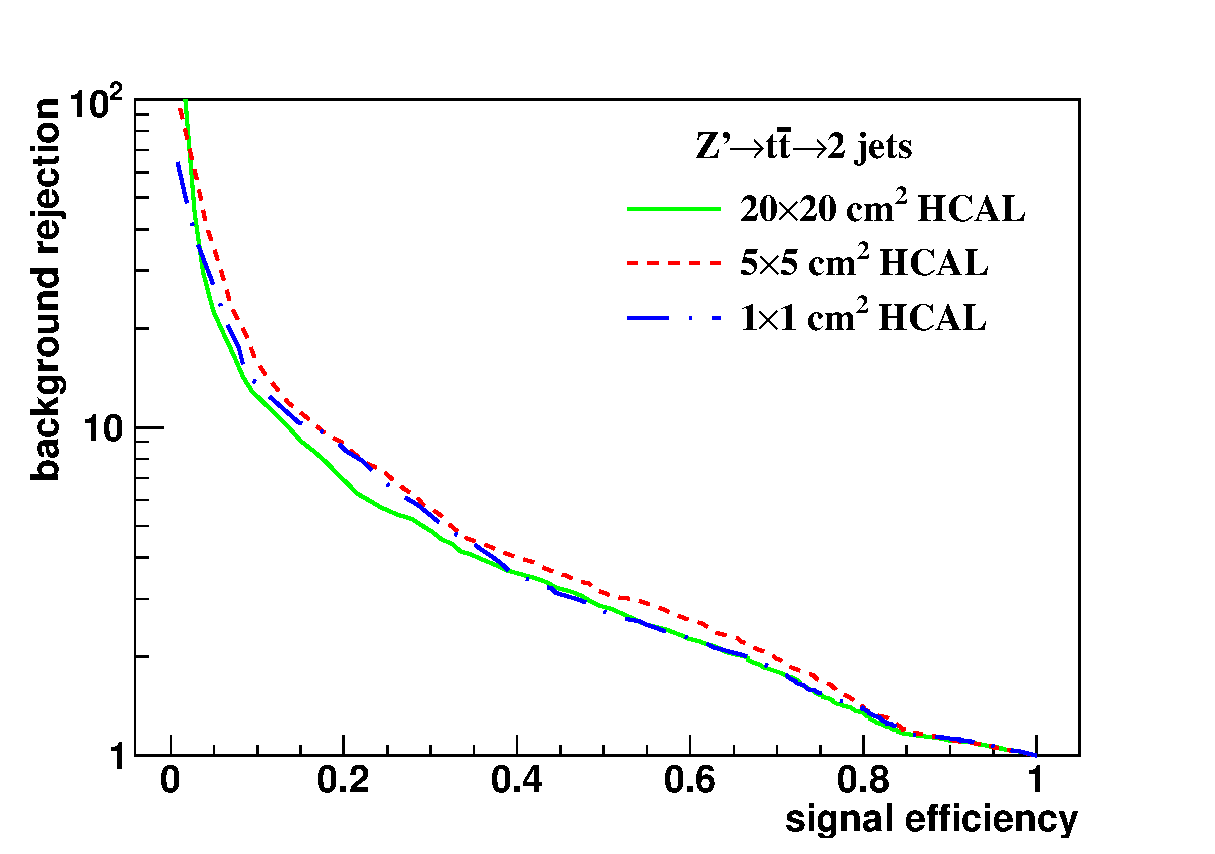
\includegraphics[  width=0.45\textwidth]{ROC_soft_drop/A_Cluster_mass_sdb2_40tev_eff_1_central_fix_at_Median_bin_tt_qq_log_no_UOF.eps}
 }
\end{center}
\caption{
The ROC curves of soft drop mass selection for $\beta=2$
with resonance masses of 5, 10, 20 and 40 TeV. 
Three different detector cell sizes are compared: 20~$\times$~20, 
5~$\times$~5 and 1~$\times$~1 cm$^2$. 
The signal (background) process is $Z'\rightarrow t\bar{t}$
($Z' \rightarrow q\bar{q}$).
}
\label{fig:cluster_mass_sdb2_tt_ROC}
\end{figure}

These studies show that the reconstruction of soft drop mass improves with decreasing  HCAL cell sizes.
Figures~\ref{fig:cluster_mass_mmdt_ww_ROC} and 
\ref{fig:cluster_mass_mmdt_tt_ROC} show that for $\beta=0$ the 
smallest detector cell size, 
$1\times1$~cm$^2$, has the best separation power at 
resonance masses of 5, 10, and 20~TeV when the signal is the $Z' \rightarrow WW$ process,  and 
at  resonance masses of 10 and 20 TeV when the signal is the $Z' \rightarrow t\bar{t}$ process.
However, for $\beta=2$, Figs.~\ref{fig:cluster_mass_sdb2_ww_ROC} and \ref{fig:cluster_mass_sdb2_tt_ROC} 
show that the smallest detector cell size 
does not have improvements in the separation power when compared with 
larger cell sizes. In fact, the performance for the three cell sizes is  
similar. 

Note that the separation between ROC curves depends 
on the physics variable and on the boost of the top quarks or the $W$ bosons. For example, 
the similarity between the ROC curves shown in Fig.~\ref{fig:cluster_mass_mmdt_tt_ROC}(a)
is due to the insufficient boost of the top quarks, 
 where even the largest cell size provides adequate discrimination from unstructured jets.
On the other hand, Fig.~\ref{fig:cluster_mass_mmdt_tt_ROC}(d) does not show a difference 
between the ROC curves because the boost is too high,  where even the smallest  cell size is not small enough, or the lateral spreading of the particle showers 
 prevents discrimination from unstructured jets. For both $Z' \to WW$ and $Z' \to t \bar{t}$ processes at $M(Z’) = 40$~TeV, the typical opening angle between the daughter jets 
 is 17 mrad or less; the smallest cell size we consider (1~$\times$~1~cm$^2$ or $\Delta \eta \times \Delta \phi = 0.0043 \times 0.0043$) 
 is not able to distinguish the substructure at this angular scale.  

We also find that the  soft drop mass with $\beta=0$ has better 
performance for distinguishing signal from background than with  $\beta=2$. Therefore, we will 
apply requirements on the soft drop mass with $\beta=0$  when studying the other jet substructure 
variables. 
 
